\documentclass[withindex,glossary, oneside]{cam-thesis}
% \documentclass[oneside]{book}
% Citations using numbers\documentclass{standalone}
\usepackage[T1]{fontenc}     
\usepackage[toc,page]{appendix}
\usepackage{tikz}
\usepackage{tikz-qtree,tikz-qtree-compat}
\usetikzlibrary{calc}
\usepackage{multirow}
\usepackage{array}
\usepackage[utf8]{inputenc}             
\usepackage{tikz}
\usepackage{float}
\usepackage{forest}
\usepackage{blindtext}
\usepackage{tabularx}
\usepackage{subfigure}
\usepackage{pgfplots}
\pgfplotsset{compat=1.14}
\usepackage[utf8]{inputenc}
\usepackage{amsmath, amssymb, latexsym}
\usepackage{tikz}
\usetikzlibrary{decorations.pathreplacing}
\usetikzlibrary{fadings}
\usetikzlibrary{shapes,arrows,fit,calc,positioning}
\tikzset{box/.style={draw, diamond, thick, text centered, minimum height=0.5cm, minimum width=1cm}}
\tikzset{line/.style={draw, thick, -latex'}}
% FOR MATHS
\usepackage[numbers]{natbib}
\usepackage{amsmath}
\usepackage{amssymb}
\newcommand{\R}{\mathbb{R}}
\newcommand{\argmax}{\arg\!\max}
% FOR ALGORITHMS
\usepackage{algorithm}
\usepackage[noend]{algpseudocode}

\title{Comparing Machine Learning Techniques for Mobility
Graph Classification}
\author{Miteyan Patel}
% \college{Robinson College}
% \collegeshield{CollegeShields/Robinson}
% \submissiondate{20th May, 2018}
% \date{May, 2018}
% \subjectline{Computer Science}
\begin{document}
% \frontmatter{} 
\pagestyle{empty}
\rightline{\LARGE \textbf{Miteyan Patel}}
\vspace*{60mm}
\begin{center}
\Huge
\textbf{Comparing Machine-Learning Techniques for Mobility Graph Classification} \\[5mm]
Computer Science Tripos -- Part II \\[5mm]
Robinson College \\[5mm]
\today  % today's date
\end{center}
% Proforma, table of contents and list of figures
\pagestyle{plain}
\chapter*{Proforma}
{\large
\begin{tabular}{ll}
Name:               & \bf Miteyan Patel                       \\
College:            & \bf Robinson College                     \\
Project Title:      & \bf Comparing Machine-Learning Techniques for\\&\bf Mobility Graph Classification\\
Examination:        & \bf Computer Science Tripos -- Part II, June 2018  \\
Word Count:         & \bf 11891\footnotemark[1]\\
Project Originator: & \bf Dr S.~Servia                    \\
Supervisor:         & \bf Dr S.~Servia                    \\ 
\end{tabular}
}
\footnotetext[1]{This word count was computed by TeXcount}

\stepcounter{footnote}
\section*{Original Aims of the Project}
This project aims to investigate supervised machine learning algorithms for graph classification. Specifically, we are interested in graphs that represent users' mobility patterns which can be obtained from spatio-temporal data gathered with their smartphones. The evaluation of these algorithms is performed both on synthetic and spatio-temporal datasets. The best performing model is then to be incorporated to an Android application to infer users’ demographics from their mobility patterns.

\section*{Work Completed}
The dissertation was a success, meeting and extending the requirements. I have created graphs representing the mobility of users from the spatio-temporal datasets provided as well as a synthetic dataset. Then I applied  and evaluated several supervised learning algorithms, including Naive Bayes, Decision Trees, Random Forests, Support Vector Machines, MLPs, the CNN on Graphs with Fast Localized Spectral Filtering implementation and my own MLP implementation in Java. The best performing model trained using a real-world dataset was exported to an Android Application to infer several demographic variables such as gender and occupational status of the user based on their movement.
\section*{Special Difficulties}
None.
\section*{Declaration}
\thispagestyle{empty}
I, Miteyan Patel of Robinson College,
being a candidate for Part II of the Computer Science Tripos,
hereby declare that this dissertation and the work described in it
are my own work, unaided except as may be specified below, and
that the dissertation does not contain material that has already
been used to any substantial extent for a comparable purpose.\\
Signed:
Miteyan Patel\\
Date: 18/4/2018

% Leaving some space for the signature:
\vspace{15mm}
\begin{flushright}
Miteyan Patel\\
May, 2018\\
\end{flushright}
\vfill

\tableofcontents
%% Thesis body:
%%
\chapter{Introduction}
\section{Motivation}
Machine-learning techniques typically use structured, organised data, which restricts the domain of data that can be used. Unstructured data such as graphs do not have a pre-defined data model and arise commonly, for example in the domain of social and web networks and bioinformatics. Consequently, graph classification algorithms would open access to using vast amounts of currently unusable unstructured data.
An interesting problem is the classification of \textit{mobility graphs}, where the nodes correspond to the locations visited by the user and edges as transitions between these locations. 
This could be used for early detection of Alzheimer’s Disease from alterations in the movement patterns of its sufferers. The prominent prevalence of mobile phone usage allows us to ethically monitor and analyse users' locations by  solely local computations on the users' smartphones. 

On-device machine learning has massive potential in the mobile domain. For example, optimising battery life through intelligent task management utilising usage patterns of the users applications~\cite{androido}, or to detect user well-being~\cite{well-being}. Furthermore, an external centralised server for data processing is no longer needed, eliminating concerns over the leaking of sensitive data over the network or through security flaws and also reducing data protection legislation concerns.
\section{This Project}
This dissertation details the development of an Android application that is capable of locally inferring the demographic class of its user. Mobility graphs extracted from spatio-temporal datasets are used to train a collection of supervised machine-learning algorithms, including a new Convolutional Neural Network architecture~\cite{CNN1}, from which the best model, Random Forest, is trained and transferred onto the application.
The mobility graphs used for training are constructed from datasets containing user's demographic labels such as gender or occupation. The classifiers are optimised and then evaluated to determine the most suitable model to export to the application. The application collects and then clusters the location data into graphs, which are used to infer the users' demographic class, in particular their type of occupation. This project has the potential to impact the design of future applications for location tracking and classification analysis. \\
\section{Related Work}
Smart phones already use machine learning locally to do various tasks from predictive typing on keyboards to classifying images into folders and making suggested actions of highlighted text~\cite{androido}. Wearable technology like smart watches also make use of passive data collected from the sensors throughout the day to infer step counts, heart rate or even if the user could have an underlying disease~\cite{apple}.

Regarding the machine learning algorithms used, CNNs~\citep{CNN1} have been applied to classify images, natural language texts, random synthetic graphs. However, to our knowledge, its application for mobility-graph classification is still to be investigated.\\
\chapter{Preparation}
My preparation consisted of learning about supervised machine-learning algorithms in order to optimize them for the task of mobility-graphs classification. Understanding techniques for evaluating the machine-learning algorithms was paramount in ensuring that the correct algorithm is chosen. Research in graph theory was done to find the most relevant features that could be used to classify graphs and to find techniques such as clustering to create the graphs from the raw location data. This chapter contains the algorithms used for clustering, graph feature extraction, supervised classification algorithms and software engineering practices used. 
\section{Clustering}
Location data needs to be grouped so that close together recordings are in the same cluster, which represents a single place the user has visited. Clustering will reduce the number of locations visited in the graph and increase the edge weight between the nodes. That makes the graphs simpler to process whilst conveying more information through greater edge weights than a graph simply representing each location as a node. 

Clustering involves grouping data into sets in such a way that objects in the same group are more similar to each other than to those in other groups. 
A useful algorithm for spatial clustering is the DBSCAN algorithm. It is efficient enough to work on Android phones. It also does not need the number of clusters to be specified as with k-means clustering, which is an ambiguous problem and depends on the data set.
\subsection{Density-Based Spatial Clustering Of Applications With Noise}
DBSCAN is a clustering algorithm described in Algorithm 1. Given a set of points in space, it groups together points with many nearby neighbours in a cluster, and marks distant points as noise. It takes two parameters, a minimum distance a point needs to be from another point to be considered its neighbour, $\epsilon$, and the minimum number of points needed to form a cluster, \textit{minPoints}. 
If there are more than \textit{minPoints} other points within $\epsilon$ from a random point, a cluster is formed. The cluster is expanded by checking the new points and if they have more than \textit{minPoints} points within $\epsilon$ the cluster is grown recursively. The process is repeated until the cluster cannot be expanded. A point with fewer than \textit{minPoints} is considered as an outlier or "noise point" and does not belong to any cluster.
% Mention figures, algorithms, and tables with capitals. 
\begin{algorithm}
\caption{DBSCAN algorithm for clustering locations}
\label{alg:erdos}
\begin{algorithmic}[1]
\Procedure{$cluster(locations, \epsilon, minPoints)$}{}
\State clusters = []
\For {randomLocation in unvisited(locations)}
\State cluster = $\emptyset$
		\While {numNeighbours(randomLocation, $\epsilon$) > minPoints}
        	\State $cluster \gets neighbours(randomPoint, \epsilon)$
            \State $randomLocation \gets cluster.nextPoint$
        \EndWhile
		\State $clusters \cup cluster$
\EndFor
\State \textbf{return} clusters
\EndProcedure
\end{algorithmic}
\end{algorithm}

\section{Graph Theory}
A graph $G$ can be defined as a pair $(V,E)$, where $V$ is a set of vertices, and $E$ is a set of edges between the vertices. To use graphs constructed from the user location data as input into the traditional supervised machine learning algorithms, features must be extracted from the graphs. I explain some of the features we can extract to distinguish between graphs belonging to different classes. Some of these features are vectors defined for each node in the graph, in this case the mean and variances of these vectors are used as features. The vectors of these features themselves could be used for this. However, each graph would then need to be reduced to the same size and the vectors sorted on a particular metric such as the nodes degree. This is left as future work. 
\subsection{Graph Features}
\begin{description}
\item [Number of nodes and edges:] of the graph.
\item [Maximum degree:] the maximum number of neighbours any node in the graph has.
\item [Density:] defined as: $$\frac{|Edges|}{|Nodes|(|Nodes| - 1)}$$ for directed graphs, a dense graph has the number of edges close to the maximal number of edges possible. 
\item [Eccentricity:] of a node is the maximum distance to any other node in the graph. This is a vector defined for each node in the graph and so the mean and variance of the eccentricity are used as two separate scalar features.
\item [Diameter:] the maximum eccentricity value.
\item [Radius:] the minimum eccentricity value.
\item [Centre Size:] the size of the centre of a graph. The centre of a graph is the set of all nodes in the graph which have eccentricity equal to the radius of the graph. 
\item [Shortest Path Length:] the average and variance of the shortest path between all pairs of nodes in the graph. 
\item [Clustering Coefficient:] measure of the degree to which nodes in a graph tend to cluster together. 
\item [Betweenness Centrality:] for each vertex is the number of all pair shortest paths that pass through it. The shortest path between two vertices is one where the sum of the edge weights in the path is minimised.
\item [Edge-Betweenness Centrality:] vector containing the fraction of shortest paths each edge belongs to. The mean and variance of these are extracted as features.
\item [PageRank:] computes a ranking of the nodes in the graph based on the structure of  incoming links.
\end{description}
\section{Supervised Machine Learning}
Supervised learning algorithms are used to learn the mapping function from input data to its class. Input feature vectors $\mathbf{x} \in \R^{m}$ are associated with a class $y$. In classification problems, $y$ represents one of the possible output classes $\mathbf{C} = \{C_1, ..., C_k\}$.
 A training set is composed of $n$ such training examples: $$\mathbf{s} = [(\mathbf{x_1}, y_1) (\mathbf{x_2}, y_2) ... (\mathbf{x_n}, y_n)]$$
The goal is to approximate the mapping function, the hypothesis $h:  \R^{m} \rightarrow \mathbf{C}$, so for new input data $\mathbf{x}$, the output class for that data can be predicted. The following sections explain the theory behind the machine-learning techniques I use.
\subsection{Naive Bayes Classifier}
Naive Bayes classifier is a simple probabilistic classifier based on applying Bayes' theorem with the assumption between the features are independent. This is the major problem with this approach, since features derived from the graphs are likely dependent on each other. An advantage of Naive Bayes is that it only requires a small amount of training data to estimate the parameters necessary for classification.
Bayes' theorem states describes the likelihood of an event $A$ given an event $B$ is true probability, based on prior knowledge of conditions that might be related to the event. 
$$ P(C_k \mid \mathbf{x}) = \frac{P(\mathbf{x} \mid C_k) \, P(C_k)}{P(\mathbf{x})} $$
In reality only the numerator is of interest since the denominator does not depend on the class $\mathbf{C}$ so it is effectively a constant and can be discarded: 
\begin{equation}
\begin{split}
{P(C_k, x_1, x_2, ..., x_n)} & = P(x_1 \mid C_k, x_2, ..., x_n)P(x_2, ... , x_n, C_k) \\
% 							  & = P(x_1 \mid C_k, x_2, ..., x_n)P(x_2 \mid x_3, ... , x_n, C_k)P(x_3, ... , x_n, C_k) \\
%                               & = ...\\
                              & = P(x_1 \mid C_k, x_2, ..., x_n)...P(x_n-1 \mid x_n, C_k)P(x_n \mid C_k)P(C_k)
\end{split}
\end{equation}
Using the naive assumption that each feature ${x_i}$ is conditionally independent we have:
\begin{equation}
\begin{split}
P(x_i \mid x_{i+1}, ..., x_n, C_k) = P(x_i \mid C_k)
\end{split}
\end{equation}
Therefore, the conditional probability of the class variable $C$ is:
\begin{equation}
\begin{split}
{P(C_k, x_1, x_2, ..., x_n)} & \propto P(C_k){\displaystyle \prod_{i=1}^{n} P(x_i \mid C_k)}
\end{split}
\end{equation}
Finally, to construct the naive Bayes classifier the most probable hypothesis is chosen known as the maximum a posteriori decision rule and the corresponding Bayes classifier is the function that assigns a class label $\hat y = C_k$, for some class $C_k$ as:
\begin{equation}
\begin{split}
\hat y = \argmax_k  P(C_k){\displaystyle \prod_{i=1}^{n} P(x_i \mid C_k)}
\end{split}
\end{equation}
\subsection{Support Vector Machines}
Support Vector Machines represent training data as points in space and are mapped so that the examples of the separate categories are divided by a margin that is as wide as possible. When new examples are observed they are mapped into that same space and predicted to belong to a category based on which side of the gap they fall. SVMs can efficiently perform a non-linear classification, mapping their inputs into high-dimensional feature spaces, known as the kernel trick. They work by finding a dividing hyperplane which maximises the distance between the closest points between the classes to the hyperplane as seen in Figure \ref{fig:svm}. 
  \tikzset{
    leftNode/.style={circle,minimum width=.5ex, fill=none,draw},
    rightNode/.style={circle,minimum width=.5ex, fill=black,thick,draw},
    rightNodeInLine/.style={solid,circle,minimum width=.7ex, fill=black,thick,draw=white},
    leftNodeInLine/.style={solid,circle,minimum width=.7ex, fill=none,thick,draw},
  }
  \begin{figure}[H]
\centering
  \begin{tikzpicture}[
        scale=2,
        important line/.style={thick}, dashed line/.style={dashed, thin},
        every node/.style={color=black},
    ]
    \draw[dashed line, yshift=.7cm]
       (.2,.2) coordinate (sls) -- (2.5,2.5) coordinate (sle)
       node[solid,circle,minimum width=2.8ex,fill=none,thick,draw] (name) at (2,2){}
       node[leftNodeInLine] (name) at (2,2){}
       node[solid,circle,minimum width=2.8ex,fill=none,thick,draw] (name) at (1.5,1.5){}
       node[leftNodeInLine] (name) at (1.5,1.5){}
       node [above right] {$w\cdot x + b > 1$};

    \draw[important line]
       (.7,.7) coordinate (lines) -- (3,3) coordinate (linee)
       node [above right] {$w\cdot x + b = 0$};

    \draw[dashed line, xshift=.7cm]
       (.2,.2) coordinate (ils) -- (2.5,2.5) coordinate (ile)
       node[solid,circle,minimum width=2.8ex,fill=none,thick,draw] (name) at (1.8,1.8){}
       node[rightNodeInLine] (name) at (1.8,1.8){}
       node [above right] {$w\cdot x + b < -1$};

    \draw[very thick,<->] ($(sls)+(.2,.2)$) -- ($(ils)+(.2,.2)$)
       node[sloped,above, near start] {};

    \foreach \Point in {(.9,2.4), (1.3,2.5), (1.3,2.1), (2,3), (1,2.9)}{
      \draw \Point node[leftNode]{};
    }

    \foreach \Point in {(2.9,1.4), (2.3,.5), (3.3,.1), (2,0.9), (2.5,1)}{
      \draw \Point node[rightNode]{};
    }
  \end{tikzpicture}
\caption{A visualisation of the hyperplane that splits the two classes with a maximum distance between any point in the classes to maximum margin.} \label{fig:svm}
\end{figure}

\subsubsection{Kernel Functions}
Kernels are functions that allow the computation of a cross product in the larger feature space without explicitly calculating the coordinates in that space or knowing that space. This is computationally cheaper than the explicit computation of the coordinates and allows for the input feature vectors to be mapped onto a higher-dimensional space for a finding a better hyperplane. The choice of the kernel function determines the quality of the classifiers, popular kernel functions are: 
\begin{itemize}
\item Linear kernels; these are equivalent to the standard cross product between the data inputs $\mathbf{x}_i$ and $\mathbf{x}$ with an additional optional parameter $c$: $$k(\mathbf{x}_i,\mathbf{x}) = \mathbf{x}_i \mathbf{x}^\mathsf{T} + c$$
\item Polynomial kernels; these are represented with adjustable parameters for the slope $\alpha$, constant term $c$, and polynomial degree $d$: $$k(\mathbf{x}_i,\mathbf{x}) = (\alpha \mathbf{x}_i \mathbf{x}^\mathsf{T} + c)^{d}$$
\item Sigmoid function; this was also used and is the same as the sigmoid activation function used in the neural networks. It also uses adjustable parameters for the slope $\alpha$ and a constant term $c$: 
$$k(\mathbf{x}_i,\mathbf{x}) = \tanh(\alpha \mathbf{x}_i \mathbf{x}^\mathsf{T} + c)$$
\end{itemize}
% \subsubsection{Decision Boundary}
% The decision boundary shape represents the number of classifiers to train. One vs rest trains one classifier per class. This often leads to imbalanced datasets meaning generic SVM might not work, but still there are some workarounds.
% In one vs one a separate classifier is trained for each different pair of labels. This leads to $N(N-1)/2$ classifiers. This is much less sensitive to the problems of imbalanced datasets but is more computationally expensive.

\subsection{Decision Trees}
The goal is to create a model that predicts the value of a target variable by learning simple decision rules inferred from the data features. It allows the model to be visualised so the results can be more easily reasoned about compared to other machine-learning algorithms. However, the trees are prone to learn the specific training examples, known as overfitting, particularly if the tree is deep. A rooted tree is constructed with each branch containing observations about the item of data. The observations are used to traverse down the tree until the conclusion about the data is retrieved at the leaf nodes of the tree. 
Figure \ref{fig:decision} is a decision tree where $o_i$ are observations and $C_i$ are classes. Classes are inferred by traversing the tree from the root observation to the leaves which are the classes.
\begin{figure}[H]
$$\begin{forest}
for tree={l sep+=.8cm,s sep+=.5cm,shape=rectangle, rounded corners,
    draw, align=center,
    top color=white, bottom color=gray!20}
  [$o_0$
     [$o_1$,for children={font=\bfseries},edge label={node[midway,left]{$\checkmark$}} 
       [$C_0$, edge label={node[midway,left]{$\checkmark$}} ]
       [$C_1$, edge label={node[midway,right]{$\times$}}]     
     ]
     [$o_2$,font=\bfseries,edge label={node[midway,right]{$\times$}} 
       [$o_3$,for children={font=\bfseries}, edge label={node[midway,left]{$\checkmark$}}
         [$C_0$, edge label={node[midway,left]{$\checkmark$}} ]
         [$C_1$, edge label={node[midway,right]{$\times$}}]       
       ]
       [$o_4$, for children={font=\bfseries}, edge label={node[midway,right]{$\times$}}
       [$C_1$, edge label={node[midway,left]{$\checkmark$}} ]
       [$C_2$, edge label={node[midway,right]{$\times$}}]]
     ]
]    
\end{forest}
$$
% remove tree.
\caption{Example Decision Tree diagram}
\label{fig:decision}

\end{figure}
\subsection{Random Forests}
Random forests are an ensemble of decision trees. Random forests prevent overfitting experienced by single decision trees by constructing many different decision trees using only certain subset of the feature vector during training. Overall, although each tree will only incorporate a small random subset of features, collectively most or all of the features will be used by all of the trees. This randomness prevents highly correlated trees since a few features that are particularly predictive could be used to construct the trees with a small training error, but may not generalise well to new examples. The modal class that of all the decision trees is used for the class inference.
\subsection{Neural Networks}
Based on the extravagantly complex neuron networks in the brain, neural networks, offer a commonly used technique for regression and classification problems. 
The goal is to define a function $f(\mathbf{x};\mathbf{w}, \mathbf{b}$), to approximate the hypothesis function, where $\mathbf{x}$ is the input vector, $\mathbf{w}$ and $\mathbf{b}$ are the weights and biases in the network.During the training phase the values of weights and biases that minimise a loss function are learnt. A loss function defines the measure of the error when estimating $y$ from $\mathbf{x}$ to its actual class. The following sections describe the components of the Neural Network. \\
\subsubsection{Perceptron}
A perceptron, shown in Figure \ref{fig:Perceptron}, on its own is a linear classifier which makes predictions based on a linear combination of the weights and input features. The output of the perceptron result of the activation function applied to the the cross product between the weights and input. The constant-valued input 1 for $x_0$ is known as a bias input, which is weighted by a bias weight variable, $w_0$. This allows the output to be shifted which allows for a larger range of values. 
$$
h(w; x)= \sigma (\sum_{i=0}^{n}w_i x_i) = \sigma (\bf{w}^T \bf{x})
$$

\tikzset{basic/.style={draw,text width=1em,text badly centered}}
\tikzset{input/.style={basic,circle}}
\tikzset{weights/.style={basic,rectangle}}
\tikzset{functions/.style={basic,circle}}
\begin{figure}[H]
\centering
$$
\begin{tikzpicture}
\node[functions] (center) {};
\node[below of=center,font=\scriptsize,text width=4em] {Activation function $\sigma$};
\draw[thick] (0.5em,0.5em) -- (0,0.5em) -- (0,-0.5em) -- (-0.5em,-0.5em);
\draw (0em,0.75em) -- (0em,-0.75em);
\draw (0.75em,0em) -- (-0.75em,0em);
\node[right of=center] (right) {};
\path[draw,->] (center) -- (right);
\node[functions,left=3em of center] (left) {$\sum$};
\path[draw,->] (left) -- (center);
\node[weights,left=3em of left] (2) {$w_2$} -- (2) node[input,left of=2] (l2) {$x_2$};
\path[draw,->] (l2) -- (2);
\path[draw,->] (2) -- (left);
\node[below of=2] (dots) {$\vdots$} -- (dots) node[left of=dots] (ldots) {$\vdots$};
\node[weights,below of=dots] (n) {$w_n$} -- (n) node[input,left of=n] (ln) {$x_n$};
\path[draw,->] (ln) -- (n);
\path[draw,->] (n) -- (left);
\node[weights,above of=2] (1) {$w_1$} -- (1) node[input,left of=1] (l1) {$x_1$};
\path[draw,->] (l1) -- (1);
\path[draw,->] (1) -- (left);
\node[weights,above of=1] (0) {$w_0$} -- (0) node[input,left of=0] (l0) {$1$};
\path[draw,->] (l0) -- (0);
\path[draw,->] (0) -- (left);
\node[below of=ln,font=\scriptsize] {Inputs};
\node[below of=n,font=\scriptsize] {Weights};
\end{tikzpicture}
$$
\caption{A diagram of a perceptron showing the action of a cross product applied to the input vector \textbf{x} and weights \textbf{w}, followed by an activation function such as the sigmoid. } \label{fig:Perceptron}
\end{figure}
\subsubsection{Multi-layered Perceptron}
Perceptrons on their own are not powerful enough to generalise to more complex non-linear functions. A multilayer perceptron is a collection of fully connected perceptrons, consisting of input, internal hidden and output layers connected by the non-linear activation functions to generate non-linearity. Every perceptron is connected to at least another in the layer in front with a weight, shown in Figure \ref{fig:multilayer-perceptron}. Learning occurs in the perceptron by changing connection weights after processing the training data, based on the amount of error in the output compared to the expected result, through backpropagation (Section 2.3.5.5). 
\begin{figure}[H]
	\centering
	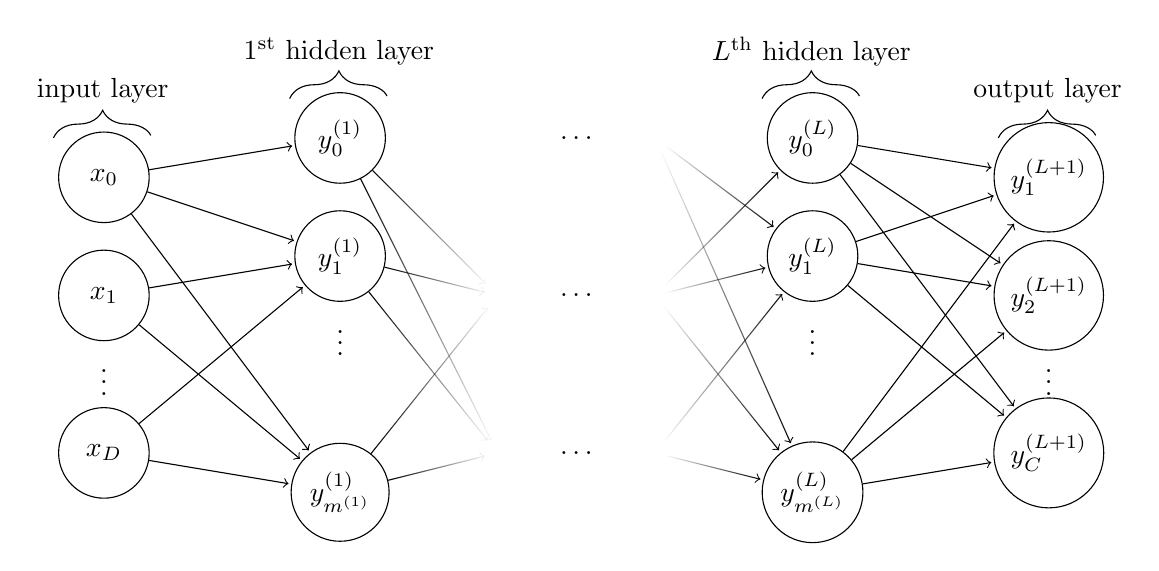
\begin{tikzpicture}[shorten >=1pt]
		\tikzstyle{unit}=[draw,shape=circle,minimum size=1.15cm]
		%\tikzstyle{hidden}=[draw,shape=circle,fill=black!25,minimum size=1.15cm]
		\tikzstyle{hidden}=[draw,shape=circle,minimum size=1.15cm]

		\node[unit](x0) at (0,3.5){$x_0$};
		\node[unit](x1) at (0,2){$x_1$};
		\node at (0,1){\vdots};
		\node[unit](xd) at (0,0){$x_D$};

		\node[hidden](h10) at (3,4){$y_0^{(1)}$};
		\node[hidden](h11) at (3,2.5){$y_1^{(1)}$};
		\node at (3,1.5){\vdots};
		\node[hidden](h1m) at (3,-0.5){$y_{m^{(1)}}^{(1)}$};

		\node(h22) at (5,0){};
		\node(h21) at (5,2){};
		\node(h20) at (5,4){};
		
		\node(d3) at (6,0){$\ldots$};
		\node(d2) at (6,2){$\ldots$};
		\node(d1) at (6,4){$\ldots$};

		\node(hL12) at (7,0){};
		\node(hL11) at (7,2){};
		\node(hL10) at (7,4){};
		
		\node[hidden](hL0) at (9,4){$y_0^{(L)}$};
		\node[hidden](hL1) at (9,2.5){$y_1^{(L)}$};
		\node at (9,1.5){\vdots};
		\node[hidden](hLm) at (9,-0.5){$y_{m^{(L)}}^{(L)}$};

		\node[unit](y1) at (12,3.5){$y_1^{(L+1)}$};
		\node[unit](y2) at (12,2){$y_2^{(L+1)}$};
		\node at (12,1){\vdots};	
		\node[unit](yc) at (12,0){$y_C^{(L+1)}$};
		
		\draw[->] (x0) -- (h10);
		\draw[->] (x0) -- (h11);
		\draw[->] (x0) -- (h1m);

		\draw[->] (x1) -- (h11);
		\draw[->] (x1) -- (h1m);

		\draw[->] (xd) -- (h11);
		\draw[->] (xd) -- (h1m);

		\draw[->] (hL0) -- (y1);
		\draw[->] (hL0) -- (yc);
		\draw[->] (hL0) -- (y2);

		\draw[->] (hL1) -- (y1);
		\draw[->] (hL1) -- (yc);
		\draw[->] (hL1) -- (y2);

		\draw[->] (hLm) -- (y1);
		\draw[->] (hLm) -- (y2);
		\draw[->] (hLm) -- (yc);
		\draw[->,path fading=east] (h10) -- (h21);
		\draw[->,path fading=east] (h10) -- (h22);
		
		\draw[->,path fading=east] (h11) -- (h21);
		\draw[->,path fading=east] (h11) -- (h22);
		
		\draw[->,path fading=east] (h1m) -- (h21);
		\draw[->,path fading=east] (h1m) -- (h22);
		
		\draw[->,path fading=west] (hL11) -- (hL0);
		\draw[->,path fading=west] (hL10) -- (hL1);
		\draw[->,path fading=west] (hL11) -- (hL1);
		\draw[->,path fading=west] (hL12) -- (hL1);
		
		\draw[->,path fading=west] (hL10) -- (hLm);
		\draw[->,path fading=west] (hL11) -- (hLm);
		\draw[->,path fading=west] (hL12) -- (hLm);
		
		\draw [decorate,decoration={brace,amplitude=10pt},xshift=-4pt,yshift=0pt] (-0.5,4) -- (0.75,4) node [black,midway,yshift=+0.6cm]{input layer};
		\draw [decorate,decoration={brace,amplitude=10pt},xshift=-4pt,yshift=0pt] (2.5,4.5) -- (3.75,4.5) node [black,midway,yshift=+0.6cm]{$1^{\text{st}}$ hidden layer};
		\draw [decorate,decoration={brace,amplitude=10pt},xshift=-4pt,yshift=0pt] (8.5,4.5) -- (9.75,4.5) node [black,midway,yshift=+0.6cm]{$L^{\text{th}}$ hidden layer};
		\draw [decorate,decoration={brace,amplitude=10pt},xshift=-4pt,yshift=0pt] (11.5,4) -- (12.75,4) node [black,midway,yshift=+0.6cm]{output layer};
	\end{tikzpicture}
	\caption[Network graph for a $(L+1)$-layer perceptron.]{Network graph of a $(L+1)$-layer perceptron with $D$ input units and $C$ output units. The $l^{\text{th}}$ inner layer contains $m^{(l)}$ inner units.}
	\label{fig:multilayer-perceptron}
\end{figure}
\subsubsection{Activation Functions}
The activation function is a non-linear function, which allows a neural network to be a universal function approximator even for a two-layered network and allows for errors to be backpropagated easily~\cite{approximator}.
\begin{figure}[H]
	\centering
	\subfigure[Logistic sigmoid]{
    		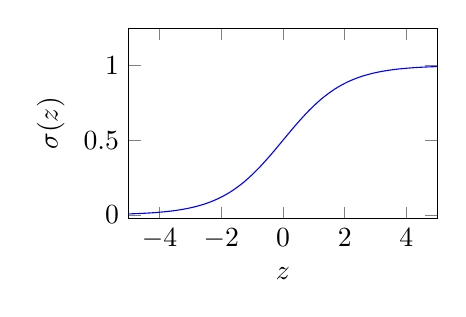
\begin{tikzpicture}
			\begin{axis}[width=5.5cm,height=4cm,ylabel=$\sigma(z)$,xlabel=$z$,ymin=-.025,ymax=1.25,xmin=-5,xmax=5]
				\addplot[blue,smooth] {1/(1+exp(-x))};
			\end{axis}
		\end{tikzpicture}
	}
	\subfigure[Hyperbolic tangent]{
		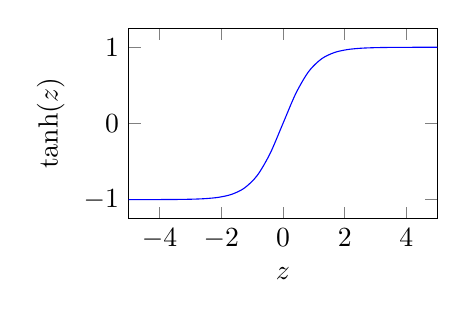
\begin{tikzpicture}
			\begin{axis}[width=5.5cm,height=4cm,ylabel=$\tanh(z)$,xlabel=$z$,ymin=-1.25,ymax=1.25,xmin=-5,xmax=5]
				\addplot[blue,smooth] {tanh(x)};
			\end{axis}
		\end{tikzpicture}
	}
    \subfigure[ReLU]{
		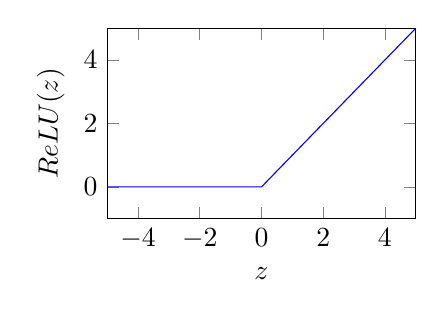
\begin{tikzpicture}
			\begin{axis}[width=5.5cm,height=4cm,ylabel=$ReLU(z)$,xlabel=$z$,ymin=-1,ymax=5,xmin=-5,xmax=5]
				\addplot[blue] {max(0,x)};
			\end{axis}
		\end{tikzpicture}
	}
    \subfigure[Leaky ReLU]{
		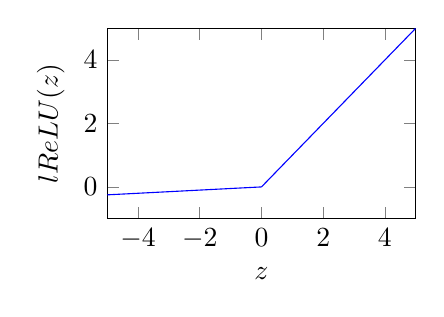
\begin{tikzpicture}
			\begin{axis}[width=5.5cm,height=4cm,ylabel=$lReLU(z)$,xlabel=$z$,ymin=-1,ymax=5,xmin=-5,xmax=5]
				\addplot[blue] {max(0.05*x,x)};
			\end{axis}
		\end{tikzpicture}
	}
    	\caption[Sigmoidal activation functions.]{Commonly used activation functions including the logistic sigmoid $\sigma(z)$, the hyperbolic tangent $tanh(z)$, ReLU and leaky ReLU.}
    	\label{fig:sigmoid-tanh}
\end{figure}
The Sigmoid function as seen in Figure \ref{fig:sigmoid-tanh} is commonly used in neural networks. 
Rectified Linear Units (ReLUs) are commonly used in CNNs, as they perform better in practice. However, for negative inputs the gradient is zero and the weights are not updated during back propagation as the derivative is undefined. This can create dead neurons, which never get activated. The leaky ReLU solves this by replacing the zero gradient section by a line with a small gradient so there are no more dead neurons for better classification. 
\subsubsection{Gradient Descent}
Gradient descent is an optimisation technique to reduce the error over the whole network to improve the mapping between the input features and the output classes. The differentiable error term $E(\mathbf{w})$ is defined, which is the squared difference between what the network is currently outputting $h(\mathbf{w,x}_i$) for the training data $\mathbf{x}_i$ and the actual class that data belongs to $y_i$:
$$
E(\textbf{w}) = \sum_{i=1}^{n} {(y_i - h(\mathbf{w};\mathbf{x}_i))}^2
$$
We try to minimise the error term for the whole network $E(\textbf{w})$ by adjusting the weights for the network $\textbf{w}$ to reduce the error by updating the weights as follows:
$$
\mathbf{w}_{t+1} = \mathbf{w}_t - \eta \frac{\partial E(\textbf{w})}{\partial \mathbf{w}}
$$
The learning rate, $\eta$, is a parameter which is a small positive number which controls the rate at which weights are updated. It is a trade-off between training time (with a large learning rate) and greater accuracy (using a smaller learning rate). In practice an adaptive learning rate is used which slowly decreases as the weights converge to reducing the error rate. This prevents getting stuck in a local minima, a sub-optimal solution. The partial differential term is the direction of the steepest decrease in error and so the weight is updated to decrease the error. For our error term where $\mathbf{x}_{i}^j$ is the jth element of $\mathbf{x}_i$ we have:
$$
\frac{\partial E(\textbf{w})}{\partial  w_j} = -2 \sum_{i=1}^{n} \mathbf{x}_{i}^j (y_i - h(\mathbf{w};\mathbf{x}_i))
$$
So the gradient-descent algorithm is as follows: initialise the weights $\mathbf{w}_0$ at the start to be random and update the weights as follows in our case:
$$
\mathbf{w}_{t+1} = \mathbf{w}_t + 2\eta  \sum_{i=1}^{n} \mathbf{x}_{i} (y_i - h(\mathbf{w};\mathbf{x}_i))
$$
We can stop once the error differences is smaller than a threshold value or a set number of iterations.
\subsubsection{Backpropagation}
The goal of backpropagation algorithm is to find a set of weights for the entire multi-layered perceptron network that minimises the error term using the gradient descent algorithm. To do this we need to find  $\frac{\partial E(\textbf{w})}{\partial \mathbf{w}}$ for the entire network which needs the calculation of $\frac{\partial E(\textbf{w})}{\partial {w}_{i,j}}$, for each weight ${w}_{i,j}$ in the network. The total error in the network produces over the entire training set is now defined as $E(\textbf{w}) = \sum_{i=1}^{n} E_i(\mathbf{w})$ and $\frac{\partial E(\textbf{w})}{\partial \mathbf{w}} =  \sum_{i=1}^{n} 
\frac{\partial E_i(\mathbf{w})}{\partial \mathbf{w}}$.
The algorithm consists of two phases, propagation and weight update:\\
\textbf{Propagation}
\begin{enumerate}
\item Propagate the input training vectors $\mathbf{x}_i$ through the network to generate the corresponding output values $h(\textbf{w};\mathbf{x}_i)$ for all nodes and the final output $y$.
\item Calculate the error term $E(\textbf{w})$ for the entire training set.
\item Propagate the actual output activations back through the network in reverse to generate the difference between the target and output values for all the neurons and weights.
% $$ or for the output layer as:
% $$
% \frac{\partial E(\textbf{w})}{\partial{w}_{i,j}^l} = \sum_{k=1}^{n} 
% \frac{\partial E_k(\textbf{w})}{\partial h(\textbf{w};\mathbf{x}_k)}  
% \frac{\partial{z}_{j}^{l+1}}{\partial{w}_{i,j}^l} 
% $$
\end{enumerate}
\textbf{Weight update}
\begin{enumerate}
\item Calculate the gradient for a weight ${w}_{i,j}^l$ in layer $l$, where ${z}_{j}^{l}$ is the output from the neuron $j$ in layer $l$, in the general case as: 
$$
\frac{\partial E(\textbf{w})}{\partial{w}_{i,j}^l} = \sum_{k=1}^{n} 
\frac{\partial E_k(\textbf{w})}{\partial h(\textbf{w};\mathbf{x}_k)}  
\frac{\partial  h(\textbf{w};\mathbf{x}_k)}{\partial{z}_{j}^{l+1}} 
\frac{\partial{z}_{j}^{l+1}}{\partial{w}_{i,j}^l} 
$$
\item Update the weights using gradient descent as before with rule:
$$
{w}_{i,j}^l := {w}_{i,j}^l - \eta \frac{\partial E(\textbf{w})}{\partial{w}_{i,j}^l} 
$$
\end{enumerate}
\usetikzlibrary{matrix,chains,positioning,decorations.pathreplacing,arrows,calc}
\tikzset{
block/.style={
  draw,
  rectangle, 
  text width=3em, 
  text centered, 
  minimum height=8mm,     
  node distance=2.3em
  }, 
line/.style={draw}
}

\subsubsection{Softmax} 
The softmax function creates a probability distribution over $K$ different possible outputs, where the $\sum_{j=1}^{K}\sigma(\mathbf{z}_j) = 1$. It is applied to the final fully connected layer to ensure the sum of the activations for all the neurons is 1 to allow inference for the most likely class. 
$$ \sigma(\mathbf{z}_j) = \frac{e^{z_j}}{\sum_{k=1}^{K} e^{z_k}}$$
\subsection{Convolution Neural Networks}
CNNs are based on the Neural Network architecture but use convolutions between the weight layers and the input features. The CNN inner or hidden layers unlike Neural Networks are composed of specific convolutional, pooling, fully connected and normalization layers. Filters are convolved over each layer which extracts useful features. Each subsequent layer is more compressed and abstract in the features it can represent until finally a fully connected layer represents the class labels. Below each layer is described, which are shown in Figure \ref{fig:cnn}.
\graphicspath{{images/}}
\begin{figure}[H]
\centering
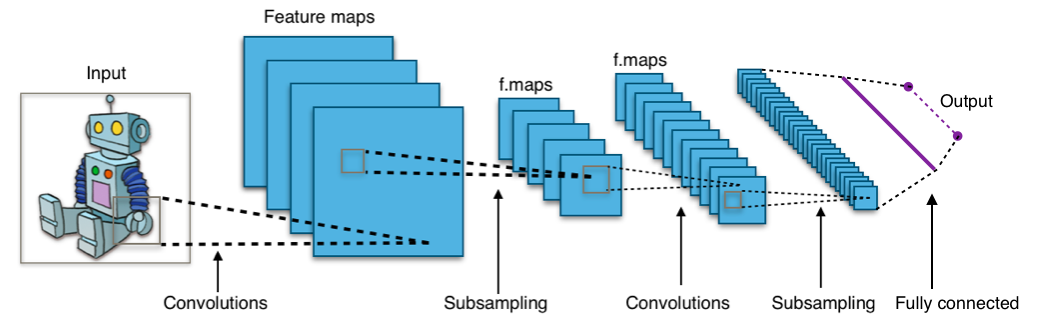
\includegraphics[scale=0.4]{cnn.png}
\caption{An example diagram of a CNN architecture showing the different layers and operations~\cite{cnn}.}\label{fig:cnn}
\end{figure}
\subsubsection{Convolutional Layer}
The convolutional layer applies a convolution operator to the input layers and the result of this is passed onto the next layer. It mimics the response of neurons to visual stimuli in their receptive fields. An activation function, typically a ReLU or Leaky ReLU is usually used after convolution operations. It adds non-linearity back into the data since convolution operations are linear and most real world data is non linear too. Using non-linear activation functions allow for a larger class of functions to be approximated.
\subsubsection{Pooling Layers}
Pooling layers are used to reduce the size of the layers. They can take multiple neurons from one layer and output a single reduced neuron to the next layer. For example, max pooling is where the maximum value of the cluster of neurons is used as the output, or average pooling where the mean average of the neuron cluster is used. It reduces the number of parameters making network more manageable, reducing overfitting and makes the network less sensitive to small input changes. 
\subsubsection{Fully Connected Layers}
A fully connected layer connects every neuron from the input layer to every neuron in the output layer. This is usually done at the output layer to get the resulting class by identifying the neuron with the largest response after the softmax function has been applied. 
\subsubsection{Training And Inference}
The overall process involves initialising the filters and weights with random values and then feeding the input data forward through the network through the convolution, ReLU, pooling and fully connected operations. The error is then calculated between the target class and predicted class with a loss function. Backpropagation is used to update all the filters and weight values to minimize the error for subsequent training steps. This is repeated for all of the training examples and allows it to generalise well towards new unseen examples. The size of the layers, parameters and filters are fixed from the start so to find out the best combinations an additional validation set can be used to optimise for the best test accuracy. 
\section{Android Application}
% services, specific android not project. APIs. Alarms, Activities, timers, Location sensors. in subheadings. This is too specific to the implementation of the app.
The Android application is built using Java and Android Studio. Android applications typically make use of the five classes detailed below:
\subsection{Activities}
\textit{Activities} interact with the user, the Activity class creates a window for the UI and be embedded inside of another activity, or can be a full-screen or floating window. Most subclasses of the Activity class implement \textit{onCreate} and \textit{onPause} methods to initialize the activity and deal with the user leaving the activity.
\subsection{View}
The \textit{View} class represents a building block for the UI. A View occupies an area on the screen and is responsible for drawing and event handling. 
\subsection{Intent}
\textit{Intents} are a passive data structure holding an abstract description of an action to be performed. They can be used to launch Activities, start Services, communicate with Services and more.
\subsection{Services}
\textit{Services} perform long-running operations in the background and continue to run in the background even if the user switches to another application.
\subsection{Alarm}
\textit{Alarms} allow the application to be run at some point in the future. When the alarm is activated the Intent registered with it is run and starts the target application. 
\section{Software Engineering}
This section deals with the requirements set out, early decisions made, tools used to deliver the project in an organised, timely fashion. Allowing me to experiment and iterate with new techniques quickly, I chose to use an iterative software development. It allows continual improvements to be made to improve the quality of the classifiers, dataset and extracted graphs.
\subsection{Implementation Approach}
Prior to development of a large-scale project such as this, it is important to break down the project. Discrete milestones, stages and tests for the project to measure progress are defined. The Android application is tested using the Android Profiler \cite{profiler} to outline the CPU and memory utilisation to ensure the application is efficient. Work begins processing the datasets and creating graphs from these. Learning algorithms were applied to the data and then these were evaluated. The best of these algorithms evaluated is exported to the Android application.
\subsection{Development}
Development work was done on my MacBook running Mac OS 10.12. Training and testing the algorithms were done on a remote server provided by the Systems Research Group to ensure no sensitive data is leaked out of the server it resides on. I used a OnePlus 5T Android smartphone with Android Oreo to test the application.
\subsection{Ethics}
Due to the sensitivity of the data contained in the datasets ethical approval from the Computer Lab ethics committee was obtained. The approval was condition on using the data solely on the private server. This is important as we are dealing with very sensitive data as well as to comply with the privacy policy that users previously signed.
\subsection{Version Control}
Version control is essential in any project of this size to organise the code base and for tracking and reverting changes made. I used Git for version control for the project code and writing the dissertation paper, these were synchronised onto a GitHub repository\footnotemark[2].
\footnotetext[2]{ \url{https://github.com/miteyan/dissertation}}

\subsection{Build Tools}
I used PyCharm for building and testing the Python code since it contains a SSH server interface for accessing the dataset stored on its private server, preventing sensitive information from leaking.\\
\subsection{Languages}
The machine-learning libraries and NetworkX were written in Python, allowing me to quickly experiment with different techniques. It was unclear if graph-feature extraction would need to be ported to the Android application since the graph CNN algorithm would not have required this. The Android application uses Java so Weka and JUNG Java libraries were used.
\section{Starting Point}
The implementation of the CNNs on Graphs with Fast Localized Spectral Filtering\citep{CNN1} was available and applied to the graphs built. There were also graphs associated with the datasets, which were used along with the DBSCAN graphs created. I was provided an Android application developed by the SRG group as part of a research project to collect location data. This was modified to prevent data being sent to the server, to allow clustering and graph-edge list formation, and run the classifier locally.\\
\subsection{Libraries}
% model brings details of real users into. Data sparsity. Not sensitive data. Eg depressed vs not is sensitive. Using graph not specific locations of the users and not leaking the users locations/houses. Why apply for ethics. Why important when using users data. could be leaking. mention throughout.
Table 2.7 contains an overview of the libraries used, the purpose and the licence for each.
\begin{figure}[H]
\begin{center}
\begin{tabular}{ |c|c|c|c| } 
 \hline
 \textbf{Library} &  \textbf{Version} & \textbf{Purpose} &  \textbf{Licence}\\ 
 TensorFlow & 1.4.0 & Deep Learning algorithms&Apache licence 2.0  \\ 
  Sci-kit Learn & 0.19.0 & Machine Learning algorithms & BSD licence \\ 
SciPy & 0.19.1& General Data management & BSD Licence   \\ 
NumPy & 1.13.1& General Data management & BSD Licence   \\ 
NetworkX &2.0 & Extracting features from graphs  & BSD licence\\ 
JUNG2 &2.0 & Extracting features from graphs  & BSD licence\\ 
WEKA & 3.8.0 & Machine Learning algorithms  & GNU licence\\ 
\hline
\end{tabular}
% caption 
\end{center}
\caption{Libraries used in the project.}
\end{figure}
\subsubsection{Licences} Apache licence 2.0 allows the user of the software the freedom to use the software for any purpose. The BSD licence requires that all code licensed from it to be licensed under the BSD licence. GNU licence  guarantees freedom to share and change all versions of the library.
\subsubsection{Graphs}
I opted for NetworkX and JUNG2, graph manipulation libraries. The key reasons are that they contain many tested, efficiently implemented graph algorithms allowing for fast prototyping and creation of graphs. JUNG2 is used on the Android platform.\\
\subsubsection{Machine Learning}
I opted for TensorFlow, Scikit-learn and Weka libraries to assist when using the machine-learning algorithms since they contain efficient, tested collections of the algorithms. \\
\subsubsection{Experience}
Figure 2.8 shows the experience prior to starting the project.
\begin{figure}[H]
\begin{center}
\begin{tabular}{ |c|c|c| } 
 \hline
 \textbf{Experience} &  \textbf{Technology or tool}\\ 
 Experienced & Java, Git, GitHub  \\ 
 Familiar & Python, Android, TensorFlow, JUnit tests\\ 
 None & Sci-kit learn, NetworkX, JUNG2, WEKA  \\ 
 \hline
\end{tabular}
\end{center}
\caption{Degrees of experience.}
\end{figure}
\section{Requirements}
The success requirements set out in the project proposal were:
\begin{itemize}
\item Training, optimising, and evaluating the performance of the supervised machine-learning algorithms on features extracted from mobility graphs.
\item Applying the CNN algorithm to the mobility graphs constructed from raw location data to classify the user into their demographic class.
\item  Evaluating the models quantitatively, then trained and ported the best performing of these onto the Android application.
\item  Implementing an Android application which can extract mobility graphs from the users location and infer the demographic class of the user locally on the device.
\end{itemize}
% CHAPTER 3
\chapter{Implementation}
In this chapter I summarise the implementation of the data preprocessing, graph constructions, training, comparison of the machine-learning algorithms and the training and porting of the best performing algorithm onto an Android application.
\section{System Overview}
The system composition is detailed in Figure \ref{fig:sys}. Clustering algorithms are applied to group together nearby locations to form the nodes and transitions between these to form the edges of the mobility graph from the spatio-temporal datasets. The graph CNN algorithm is directly applied to the mobility-graphs. Further feature extraction is done based on Section 2.2 to apply classic supervised classification algorithms as described in Section 2.3. The best classifier is then trained and incorporated to the Android application to make local inferences of the user based on their location data.
\graphicspath{{images/}}
\begin{figure}[H]
\centering
\includegraphics[scale=0.17]{sysdiagram.png}
\caption{A diagram showing the different components of the project.}\label{fig:sys}
\end{figure}
% \begin{algorithm}
% \caption{Nested Cross validation and hyperparameter training model}
% \label{alg:training}
% \begin{algorithmic}[1]
% \Procedure{$Train(model, data, parameters, k)$}{}
% \State  $split data into k folds$
% \For{k train and valid sets in training}
% 	\State  $training, test \gets k fold split(data, k) $
% \EndFor
% \EndProcedure
% \end{algorithmic}
% \end{algorithm}
\section{Spatio-Temporal Datasets}
Table 3.1 describes the datasets, preprocessing and classes inferred using the models. The datasets comprised of time and latitude-longitude pairs for each user. The models perform the classification tasks as shown in Table \ref{table:datasets}. Users whose graphs were disconnected once clustered were discarded, since not all graph features chosen are defined on disconnected graphs. Disconnected graphs can form when the user has not recorded location data consistently creating large discrepancies between location recordings creating partitions between the clusters.
\begin{table}[H]
\begin{tabular}{ |l|l|l|l| }
\hline
\multicolumn{4}{ |c| }{\textbf{Location Datasets}} \\ \hline
\multirow{1}{*}{\textbf{Input Data }} & \multicolumn{3}{ |c| }{Location and Time pairs}  \\ \hline
\multirow{1}{*}{\textbf{Preprocessed output}} & \multicolumn{3}{ |c| }{Mobility graph edge list}  \\ \hline
\multirow{1}{*}{\textbf{Dataset used}} & {MDC} & {MDC} & {EmotionSense} \\ \hline
\multirow{1}{*}{\textbf{Classification Task}} & Gender & Age & Occupation status\\ \hline
\multirow{1}{*}{\textbf{Number of users}} & \multicolumn{2}{ |c| }{157}  & 11400\\ \hline
\textbf{Classes} & {Male, Female} & 12-40, 40+ & {Full-time Employed, Other}\\ \hline
\multirow{1}{*}{\textbf{Dataset Size}} & 1209 & 493 & 6028\\
\hline
\end{tabular}
\caption{Description of datasets used along with processing, classes, sizes, duration in time per graph.}
\label{table:datasets}
\end{table}
\subsection{Mobile Data Challenge Dataset}
The Mobile Data Challenge (MDC) dataset is composed of smartphone data collected through a user study in Lausanne, Switzerland. The graphs created over a longer duration contain more information as more locations are visited. This translates to more nodes and edges in the mobility graphs for the classifiers to exploit. Therefore, the graphs were initially made for each user for each year, however this only resulted in 493 usable graphs. Many classification algorithms require more data to perform better, such as CNNs, whereas decision trees perform well enough with less data. Therefore, weekly graphs were also made to increase the count of the graph training data. 
\subsubsection{Gender Labels}
The gender distribution of the users is unbalanced, as shown in Figure \ref{fig:gender}. It is important to ensure the model is trained in an unbiased way so the lowest quality male graphs are removed to have a balanced split between the genders. Using an unbalanced labelled dataset translates to a more biased view made by the models towards the larger class, since that class holds a larger representation. In reality, genders are distributed evenly so the prediction accuracy would therefore be lower when the model is used because it would favour predicting the label that has a higher representation in the dataset.
\begin{figure}[H]
\begin{center}
\begin{tabular}{|c|c|c|} 
 \hline
 \textbf{Gender} &  \textbf{Count}\\ 
 Male & 97  \\ 
 Female & 60  \\ 
 \hline
\end{tabular}
\end{center}
\caption{Table showing the number of users with data for each gender.}
\label{fig:gender}
\end{figure}
\subsubsection{Age Labels}
\graphicspath{{images/}}
\begin{figure}[H]
\centering
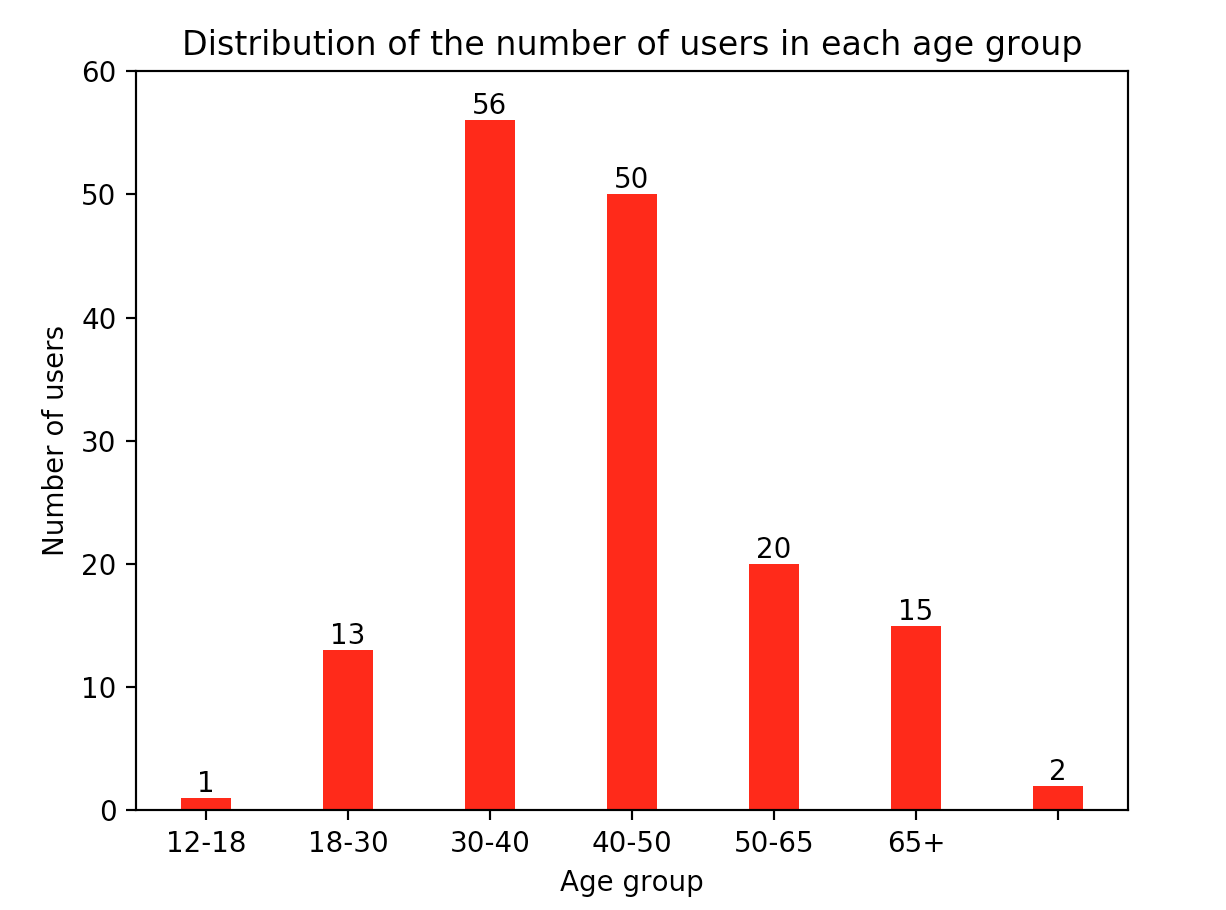
\includegraphics[scale=0.5]{hist.png}
\caption{A distribution of the number of users in each age class.}\label{fig:hist}
\end{figure}
As Figure \ref{fig:hist} shows there are two prominent age categories consisting of users aged 30-40 and 40-50 and so for a suitable split in a two-class classification problem to be consistent with the other models to allow for a fair evaluation I chose the two age classes as "less than the age of 40" and "more than 40". I also hypothesised that younger users would have different movements to older users due to differences in lifestyle and social factors so this split could have differences that the classifiers could exploit. 
\subsection{EmotionSense Dataset}
The Mobile Challenge dataset only contained demographic labels for age and gender that could be used as labels for  the graphs. The EmotionSense dataset also offered occupation data~\cite{emotion}. It could be theorized that there would be more of a variation between the graphs of users with different occupations compared to the gender or age labels as generally the employed would visit the same work place often whereas the unemployed may not have such a routine.
\subsubsection{Occupation Labels}
\graphicspath{{images/}}
\begin{figure}[H]
\centering
\includegraphics[scale=0.51]{occupation2.png}
\caption{A distribution of the number of users in each occupation group.}\label{fig:occ}
\end{figure}
As seen in Figure \ref{fig:occ} there are more users in the full-time employed occupation category and there are categories with far less users such as the home-makers and the retired. I chose a One-vs-All classifier for this problem to best exploit the amount of data we have available to prevent discarding data when balancing the dataset. Therefore, it makes sense to classify between full-time employed users and all other users as these two classes contain nearly the same number of users .

\subsection{Synthetic Graph Dataset}
Synthetic graphs are created to ensure we have graphs with statistical differences in case the graphs constructed from the datasets do not generate statistically different graphs for the labels chosen. This will allow us to determine if the techniques used in the project can successfully classify graphs.
I modify the Erdos-Renyi random graph algorithm \cite{erdos}, described in Section 3.2.3.1, which is used to create random graphs with a known probability distribution. I chose to create graphs of 50 nodes to give the classifiers more information to work whilst minimising the feature extraction and training times. 
\paragraph{The Erdos-Renyi Graph Generation Algorithm}


Erdos-Renyi algorithm, shown in Algorithm \ref{alg:erdos}, is used to create random graphs. An edge is created between two nodes randomly with the Bernoulli distribution with probability \textit{probEdge}. A simple modification allows an edge weight to be upto \textit{maxWeight}, as seen in Algorithm \ref{alg:erdos}. 
To create an edge list we simply sort the edges and use run length encoding to concatenate equivalent edges.  
\begin{algorithm}[H]
\caption{Erdos-Renyi algorithm for weighted graph edge lists}
\label{alg:erdos}
\begin{algorithmic}[1]
\Procedure{$createGraph(numNodes, probEdge, maxWeight)$}{}
\State edges = []
\For {k = [0,maxWeight]}
   \For {i = [0, numNodes]}
     \For {j = [0, numNodes]}
        \If {i != j and bernoulli(p)}
            \State $edges \gets (i, j)$
        \EndIf
     \EndFor
   \EndFor
\EndFor
\State sort(edges)
\State \textbf{return} runLengthEncoding(edges)
\EndProcedure
\end{algorithmic}
\end{algorithm}
The \textit{probEdge} used was 0.1 as that reflected the graphs from the spatio-temporal dataset the best when looking at the number of edges for the nodes. The \textit{maxWeight} was chosen to be 10 as the range of transitions between locations was in the range of 0 to 10 from the graphs constructed prior. 

\subsection{Clustering}
Clustering is used as a pre-processing step before constructing the graphs by grouping together locations from the dataset to form nodes of the graph. Clusters consist of close-together locations to signify a visited region. Using the start and end times the user was at each cluster the transitions between the clusters can be calculated to create the edge lists. I implemented the DBSCAN algorithm in Java so it also worked on the Android application. The parameters that worked for the DBSCAN in practice were using 5 metres for the \textit{minDistance} and 5 minimum nodes are needed to form a cluster. This ensures that any large building the user is in, such as at school or work, can be represented as a single node. 
\subsection{Graph Feature Extraction}
The construction of feature vectors for supervised machine learning comprised of using two libraries for retrieving the feature defined in Section 2.2.1. Initially I used the Python library NetworkX to extract the same features; however when porting to the Android Application there was no corresponding library and so Java library JUNG2 was chosen due to its ability to construct the same feature vectors. These were tested to be equal by using the same edge lists and comparing the feature vectors composed by both. \\ 
The result is a dataset composed of the feature vector and class label extracted from each graph.
\section{Supervised Machine Learning Algorithms}
The implementation of the project focused on the evaluation of the models and improving their performance. 
% The data is used for nested cross-validation, then the best hyperparameters for training the models are found, and then the evaluation metrics are computed. This allows an unbiased way to estimate hyperparameters, train and evaluate the model, while using the entirety of the available dataset, which is important due to the limited dataset size.
In the following section I detail the techniques I used to optimize the different models. 
\subsection{Hyperparameter Optimisation}
A \textit{hyperparameter} is a value set before the learning algorithm begins. All other parameters are derived via training. However we can use optimisation techniques to get a better intuition to what these values should be set to instead of guessing.
Hyperparameter optimization~\cite{hyperparameter} is the tuning of set of parameters required by a learning algorithm. It is essentially a search to find the optimal parameters by carrying out the training phase of the learning algorithm and looking for the parameters that correspond to the best performance which can be seen by the lowest loss value or best accuracies. Two common approaches used are grid search and random search.
\subsubsection{Grid Search}
Grid search involves manually specifying a list of hyperparameters and then exhaustively searching through combinations to determine the best choice of hyperparameters. This choice is good for when the range of the hyperparameters is known and to give the process guidance, therefore I used this technique with classifiers such as the SVM, Decision Tree and Random Forest since the parameters for these are mainly discrete and in a small range. However, it misses out values of hyperparameters that are not in between the parameters defined in the list provided outside the grid in favour of a smaller execution time from searching less variables.
\subsubsection{Random Search}
Random search needs a range of values each hyperparameter can take and the number of iterations to evaluate these parameters. This is a good choice when there can be a large range of values that are not intuitive to think about. I used this technique for the Neural Network implementation as there are so many values the weight neurons can take, as well as the sizes and number of layers.
\subsection{Nested Cross Validation}
Nested cross validation~\cite{nestedcrossvalidation} is used to train and test the classification algorithms with the entirety of the dataset.  This maximises the usage of the dataset whilst reducing selection bias. It involves an outer loop to split the data into training and test sets, and the inner loop is used to find the best hyperparameters of the model. Then the model is fit to these hyperparameters and then evaluated using the independent unseen test fold created by the outer loop. At the end the hyperparameters for the algorithm will be known as well as the metrics such as accuracy, loss associated with using these hyperparameters. Figure \ref{fig:nestedcv} shows the cross validation used in the project.
\graphicspath{{images/}}
\begin{figure}[H]
\centering
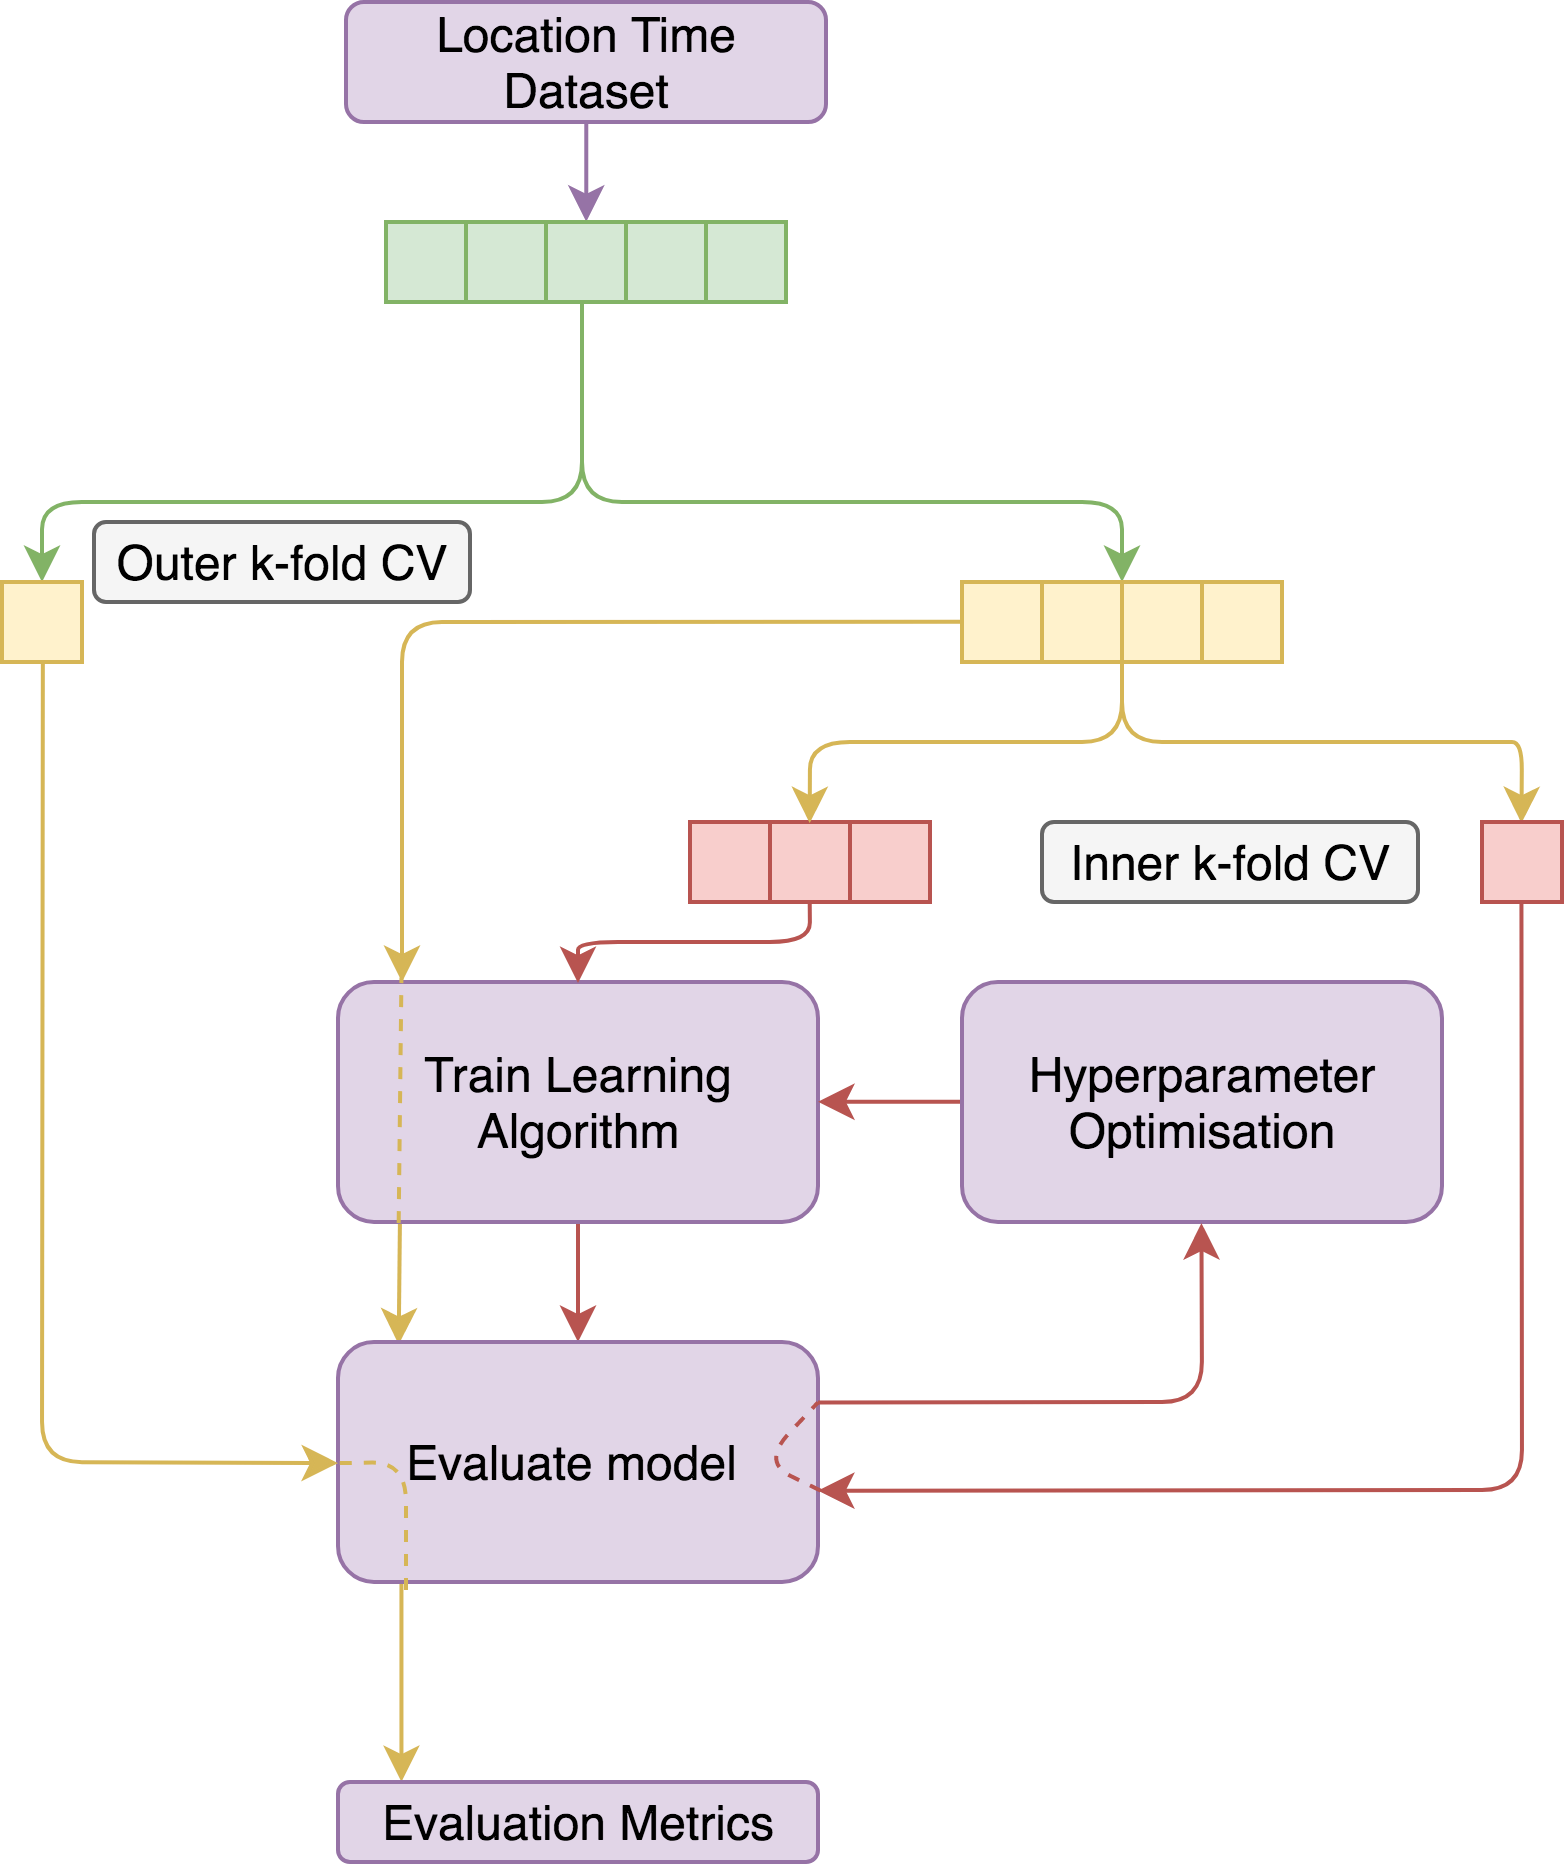
\includegraphics[scale=0.2]{nestedcv.png}
\caption{Nested cross-validation with hyperparameter optimisation.}\label{fig:nestedcv}
\end{figure}

\subsection{Feature Selection}
The data can contain features that are either redundant or irrelevant, e.g. with a low variance and can thus be removed with little loss of information. Feature selection~\cite{featureselection2} is the selection of a relevant subset of possible features for use. I used a variance-threshold method \cite{variance} in feature selection to determine that none of the features extracted from Section 2.2.1 have a normalised variance of less than 0.1.
\subsection{Feature Scaling}
The range of features extracted from the graphs vary a lot so the loss functions will not work properly since each feature will not contribute equally. Also they use multiple-dimension euclidean distance to measure the error, so it is important that all the dimensions are of equal range to prevent features with a larger range from dominating. It also allows gradient descent to converge faster.
Feature scaling~\cite{featurescaling} involves normalizing the data to have a mean of zero. This method takes into account the distribution of the features across the dataset and transforms them to a vector of a normal distribution; this can make classifiers such as the neural network train and converge faster. One formula for scaling an input feature $x$, with standard deviation $\sigma$ and mean $\mu$:
$$ x' = \frac{x - \mu}{\sigma} $$
\subsection{Overfitting}
Overfitting occurs when the model starts effectively memorising the training data with its noise. Therefore it cannot fit new unseen observations reliably and does not learn the generalisable trend. An overfitted model is a statistical model that contains more parameters or degrees of freedom than can be justified by the data. It begins to model the noise and random natural variation in the data whereas this should be ignored. Some methods used to prevent overfitting were to (i) use dropout as described in figure 3.3.7, (ii) validation datasets to stop training neural networks when the validation error stops decreasing and (iii) using appropriate parameters when training the models which can be better chosen using hyperparameter optimisation. 
\subsection{Adam Optimizer}
Adaptive moment estimation is an optimisation algorithm similar to the classical gradient descent procedure to update network weights iterative on the training data. This algorithm was used in the TensorFlow neural network.
A learning rate is kept for each of the weight parameters and is separately adapted as the learning process continues. A per-parameter learning rate improves performance on problems with sparse gradients compared to 
gradient descent as described earlier. The algorithm calculates an exponential moving average of the gradient and the squared gradient~\cite{adam}.
\subsection{Dropout}
Dropout is a regularization technique for reducing overfitting in neural networks during the training phase. It involves randomly removing hidden or visible units and their connections from the network to ensure that the network does not depend on a few units~\cite{dropout}. Therefore nodes are excluded from the net with a given probability. Only the reduced network is trained on the data in that stage. The removed nodes are then reinserted into the network with their original weights and prevents overfitting because not all of the nodes are trained on the same examples.
\subsection{Sci-kit Learn}
Sci-kit learn contains many machine-learning and data-analysis techniques to allow trying various algorithms. It was used to apply the standard classifiers including Decision Trees, Random Forests, SVMs, Naive Bayes. A nested cross-validation and metrics-gathering platform with hyperparameter optimisation was built on top. 
\subsubsection{Decision Trees}
For the Decision Tree algorithm the following hyperparameters were used: 
\textit{Maximum depth} of the tree which is used to control the size of the tree to prevent overfitting. \textit{Maximum features} is used to control the number of features from the original training set to use in the tree and are randomly selected and tried to get the best combination of features. \textit{Minimum  leaf samples} is used to control the number of samples at a leaf node. A small number will usually mean the tree is overfit to the training data, whereas a large number prevents the tree from learning the data optimally.
\subsubsection{Random Forests} Additionally to the decision tree parameters, the Random Forests also used a parameter for the number of trees in the forest.
\subsubsection{Support Vector Machines}
The hyperparameters used for the Support Vector Machines include using different kernels, decision function shapes, degrees of polynomial to use, as described in Section 2.3.2.
\subsection{Weka} 
A popular open-source library written in Java which makes it suitable for exporting to an Android application is Weka. For the graph feature vectors a Weka Instance object has to be created for input into any of the Weka classifiers. An \textit{Instance} contains a set of \textit{Attribute} objects which represents one feature from the dataset. Classes are represented with a \textit{FastVector} object. \textit{Attributes} are populated with data from the dataset to create a training set. The classifier is then created with matching hyperparameters where available and then trained. Finally this classifier is serialised and saved into a file containing the models parameters and fitted weights. This file is then saved and transferred onto the Android application, where it is de-serialised whenever a classification needs to be made. 
\subsection{TensorFlow}
TensorFlow~\cite{tensorflow} is an open-source machine learning library that I used to implement a Neural Network. TensorFlow operates on a predefined graph containing the mathematical operations required by the program and runs in a session. The TensorFlow computational graph is described by its operations on Tensor objects. A node is added to the graph for each operation used. Edges between the nodes represent the data flow of the tensors through the graph. The advantage of this representation is that it provides an easy way of understanding dependencies between the units of the computational model. It defines a low-level programming model in which the data-flow graph is defined and a TensorFlow session is run to execute the operations defined by the graph. The graph structure allows for parallelism. By using explicit edges to represent dependencies between operations, it is easy for the system to identify operations that can execute in parallel. The input to the NN the training set is defined as a rank 2 tensor, where each row consists of the input features for a training example, and the number of rows is equal to the size of the train set. A rank is the number of dimensions of a tensor.\\


The weights and biases are described as Variable objects that are trainable and maintain a persistent state across evaluations of the TensorFlow graph. Weights for each layer are represented as tensors of rank 2 and of type float32, while the biases are tensors of rank 1 and of type float32 and both are initialised to a standard normal distribution initially. It is sufficient to use float32 which is of lower precision than a 64 bit float due to faster computations and sufficient results. A layer is defined as a dictionary containing weights and biases associated with the layer and the size of its weights can be defined by the size of the number of neurons in the layer with the first layer of size as the number of features. 

\section{Convolutional Neural Networks On Graphs With Fast Localized Spectral Filtering}
The authors in \cite{CNN1} propose a new technique to learn features from the graphs that are correlated between labels to allow learning across the dataset for the classification of graphs~\cite{CNN1}. Below, I explain how I used the CNN on Graphs with Fast Localized Spectral Filtering to the problem of mobility graph classification.
\subsection{Graph Dataset Creation}
The implementation of the CNN with filtering requires a graphs adjacency matrix, which is a $N \times N$ matrix containing the number of transitions between all \textit{N} nodes in the graph, to be of the same size to allow a convolution to be applied onto them. 
\subsection{Sub-graph Extraction}
The most important \textit{N} nodes of the users' mobility graphs need to be extracted and the adjacency matrix of these nodes built. There are various metrics that define the importance of a node to the graph. These could include centrality measures such as edge or node betweenness centrality as described in Section 2.2.1. To extract a subgraph of the \textit{N} most important nodes the edge centralities of the graph is measured and the top \textit{N} most central nodes are chosen to be part of the subgraph.
\subsection{Sub-graph Size}
The problem of choosing the nodes \textit{N} to form the subgraph is important as all graphs with less than \textit{N} nodes are discarded since they do not contain enough information and this further increases the sparsity of the data available for use in the classifier. Intuitively, \textit{N} should represent the number of locations the user visits on a regular basis along with some visits to rarer locations that allow the graph to be used as a sensible representation of the different demographics, but choosing this arbitrarily is an ambiguous problem. To choose an appropriate value of \textit{ N}, the number of nodes in the subgraph, the distribution of the number of nodes in the graph dataset is extracted and \textit{N} was initially chosen as the 25th percentile of the number of nodes is extracted so 75\% of the data is kept. However, this removed a lot of information from the larger graphs by only keeping a small number of nodes and so later the median of the number of nodes in the graph dataset is kept. As seen in Figure \ref{fig:histogram} the distributions follow a decaying trend and each dataset needs a different value of \textit{N}.
\graphicspath{{images/}}
\begin{figure}[H]
\centering
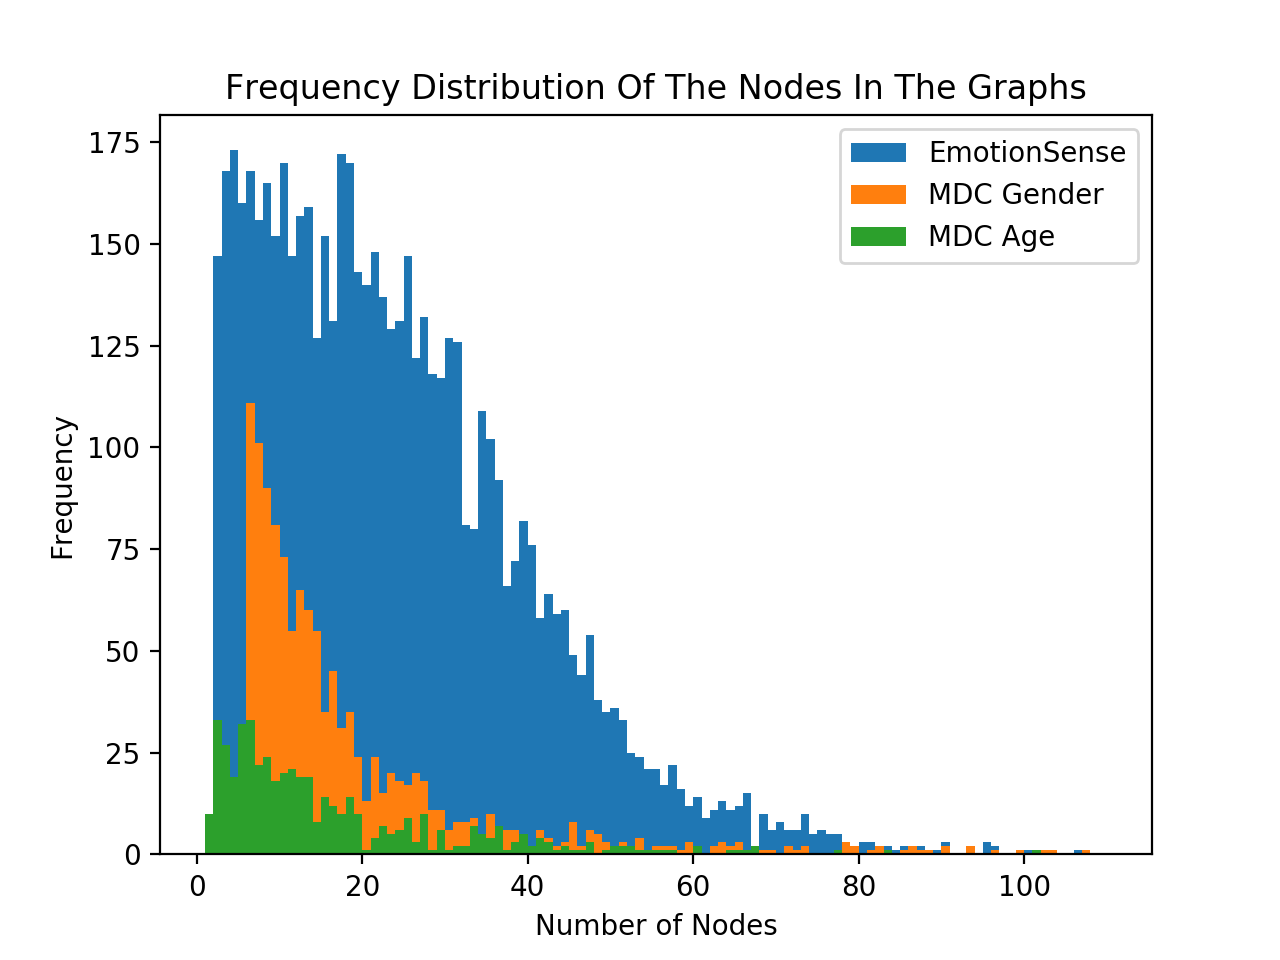
\includegraphics[scale=0.7]{graph.png}
\caption{A graph of the distribution of the number of nodes extracted from the graphs in the EmotionSense and Mobile Data Challenge datasets.}\label{fig:histogram}
\end{figure}
\subsection{CNN Model}
The CNN model is defined with a grid of parameters such as the learning rate, dropout probability, activation functions to use such as the ReLU as described in Section 2.3.5.3. The best of these are chosen using hyperparameter optimisation along with the graph signals, which are the nodes centrality measures, and the final model trained.
\subsection{Neural Network}
As an additional optional extension I implemented a multi-layered Neural Network to evaluate the differences with the popular TensorFlow implementation. To do this I implemented a Neural Network in Java and evaluated it.
\subsubsection{Class Overview}
The Neural Network is initialised to contain a specified structure of layers with a set number of neurons and a range of weights. The class overview is shown in Figure 3.7.
\graphicspath{{images/}}
\begin{figure}[H]
\centering
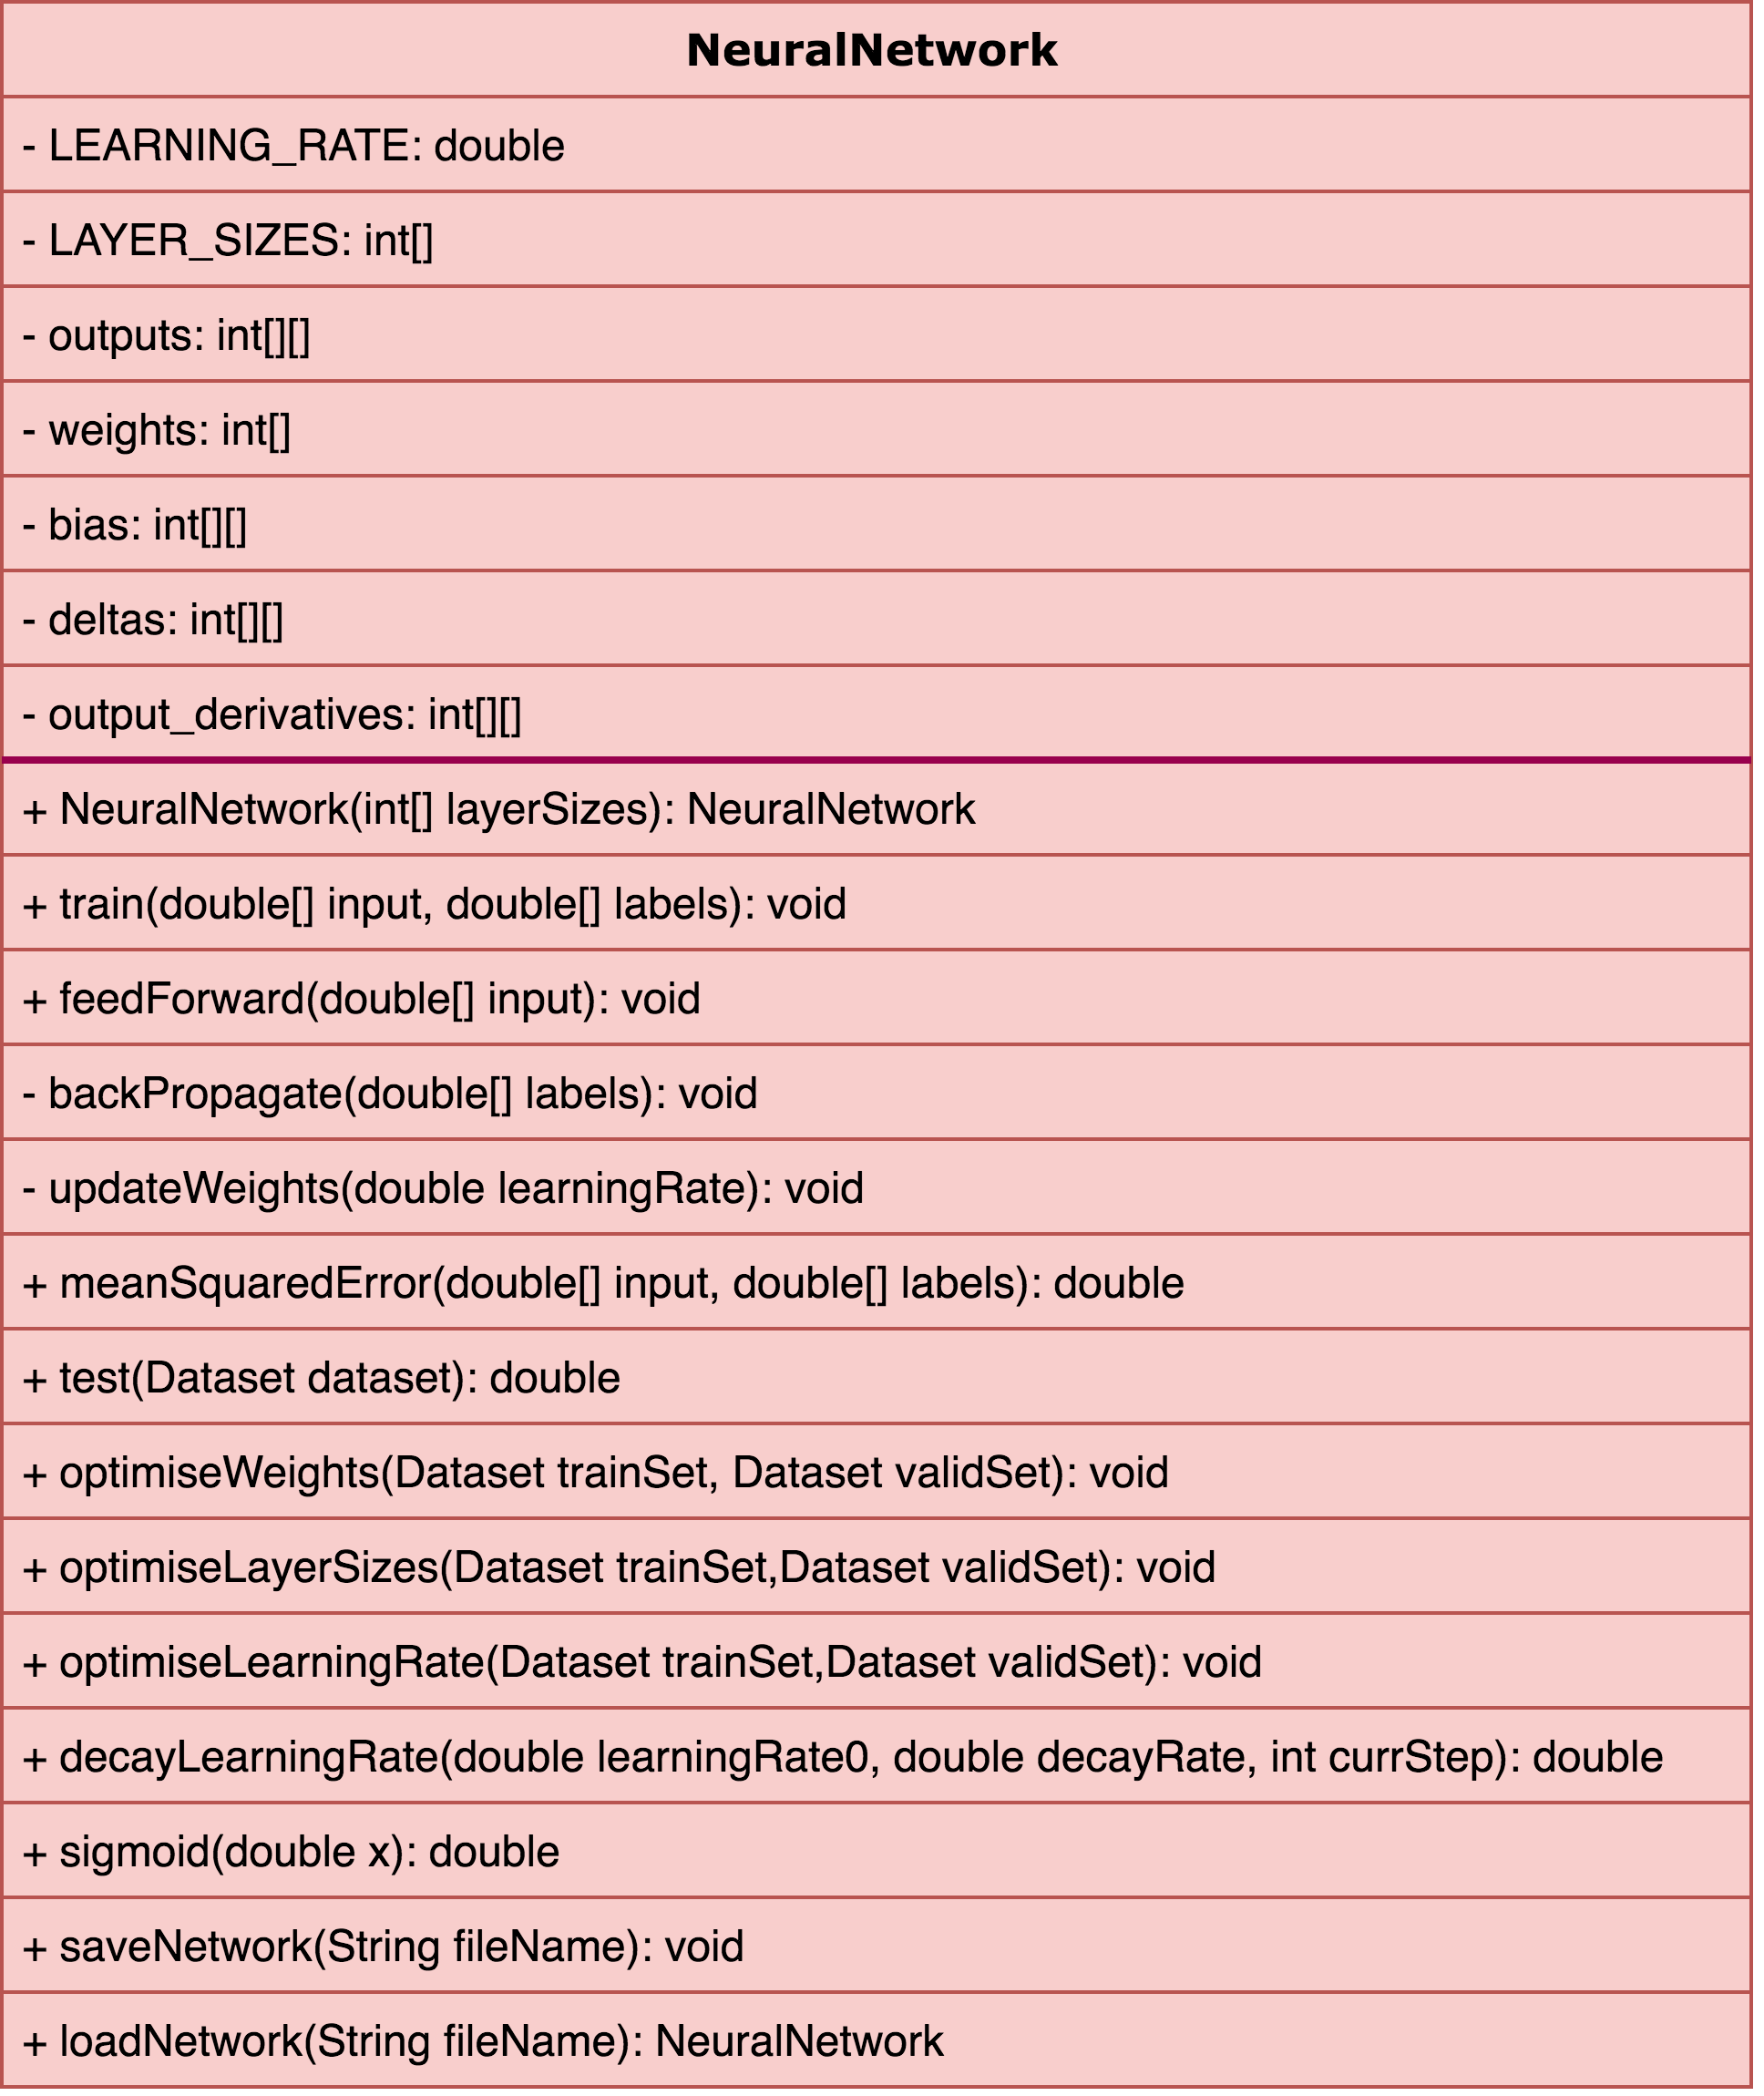
\includegraphics[scale=0.18]{nn.png}
\caption{A diagram of the Neural Network class showing the fields and methods, consisting of training and loading and saving of the network.}\label{fig:nn}
\end{figure}
\subsubsection{Training} 
Batch training is used to create sections of the train dataset to update the weights to learn the hypothesis as it is faster than using the entire dataset.
Firstly the data is fed forward through the network and derivatives calculated for the gradient descent in the backpropagation stage and the weights updated as described in Section 2.3.1. 
\subsubsection{Hyperparameter Optimisation}
Random and grid search were implemented to determine the values of the initial weights and biases, the number of layers, neurons in each layer and learning rate. This is practical for our problem since the dataset is small enough to allow a large search space of parameters to be searched but may not be applicable towards larger datasets that can take many days to train. 
\subsubsection{Testing}
To test the Neural Network written I wrote unit tests for the different components to ensure it was doing what was expected. A commonly used test is the MNIST classification task which is an optical character recognition (OCR) task from a popular dataset of handwritten images. It is a common practice in to use the MNIST dataset as a benchmark for supervised learning algorithms~\cite{MNIST}.
The MNIST dataset consists of images of handwritten characters from 0-9 and are 28x28 pixels in size. The purpose of using this dataset is to ensure the neural network can correctly classify this commonly used dataset into the 10 classes using a final set of 10 fully connected output neurons with the highest activation representing the class of the image. State-of-the-art models achieve close to 100\% accuracy. The results can be seen in Section 4.3.4.
\subsubsection{Inferring}
Once the weights have been updated a feature vector can then be propagated using the feed-forward method. This calculates the cross product between the weights and the vector. The final layer is a softmax layer to ensure the probabilities add to 1 as described in Section 2.3.1.6 and the highest valued neuron corresponds to the class inferred.
\subsubsection{Saving}
Another feature added is to save the network so that training can be done at any time and so there is no need to retrain the network from scratch every time to test it. The Java serialisable interface makes this particularly effortless as it allows the Neural Network objects to be stored into a file that can be read back as a network and so can be retrained it.

\section{Android Application}
% on-device analytics - all things are run locally on device. Mention preparation things used to build the app and the requirements. 
I incorporated the best performing machine learning model into an Android application. This application tracks the users' location to build mobility graphs locally on the device and then infer one of the classes the model is trained on. This has far-reaching consequences as it could be placed in mobile operating systems to track changes in users' behaviours and be able to detect anomalies from a change in the users' location patterns. This could be an early indicator to neurological diseases, which could be detected earlier without the need of a doctor or a formal diagnosis.
\subsection{Location Data Collection} 
To continually get location data throughout the day (even when the application is not open) a background service needs to be running which contains an alarm to schedule the collection of the location data every 30 seconds. Continuous sensing of location data is expensive in terms of battery consumption and CPU utilisation. To save battery life, Adaptive Duty Cycling is used to monitor when the user is stationary to avoid using sensors and CPU unnecessarily to waste battery and use the last collected location value instead. 
Location-time pairs are saved on a file on the device. The original application requires a user to be given an account to authenticate them, this had to be modified to prevent sensitive location data from being sent to the server. A new file is created for every week to allow a weekly graph of the data to be created and inferred. 
\subsection{Local Inferences} 
An \textit{Activity} containing the button for inferencing is started when the application is opened. A button is clicked to start the inference process by applying the DBSCAN algorithm to the location-time data collected to form the nodes. The edge list is created using the timestamps associated with the first and last value of time for the clusters. The graph features are then extracted from the edge list and the vector of features. The pre-trained exported random forest model is de-serialised on the device to infer the users' class and show the result on a new View.
\chapter{Evaluation}
In this chapter, I describe the metrics used to evaluate the algorithms and proceed to calculate the results. I present the performance of the existing language models that I implemented. I also discuss the trade-off's faced when employing those models on a mobile device. 
\section{Success Criteria}
Referring back to the success requirements set out in the project proposal:
\begin{itemize}
\item \textit{Training, optimising, and evaluating the performance of the supervised machine-learning algorithms on features extracted from mobility graphs.}\\
This criterion was exceeded, I was able to implement and apply my own neural network as extension to the datasets achieving similar results to the other learning algorithms. Many different types of mobility graphs were constructed as extensions surpassing the initial requirements.
\item \textit{Applying the CNN algorithm to the mobility graphs constructed from raw location data to classify the user into their demographic class. Evaluating the models quantitatively, then trained and ported the best performing of these onto the Android application.}\\
The CNN algorithm for graphs was applied successfully, and highlighted the  performance differences to the other classifiers. The evaluation of which is described in Section 4.3. 
\item  \textit{Evaluated the models quantitatively, then trained and ported the best performing of these onto the Android application.}\\
The algorithms have been evaluated in Section 4.3 and the Random Forest algorithm has been chosen as explained in Section 4.3.2. It has been trained on the EmotionSense dataset and ported onto the Android application.
\item  \textit{Implementing an Android application which can extract mobility graphs from the users location and infer the demographic class of the user locally on the device.}\\
The application has been tested to successfully work as described in Section 4.4. It is functional as it can apply the Random Forest algorithm on the feature vector extracted from the constructed mobility graphs locally on-device.
\end{itemize}
Meeting these criterias shows the usefulness of the application as a framework for future on-device machine learning tasks based on efficient location gathering, feature extraction and inferences.
\subsection{Extensions}
As extension my project proposal suggested to explore different constructions of graphs from the raw location data. This has been accomplished as a necessity in the implementation of the DBSCAN algorithm for clustering nodes. I was also able to create a synthetic data extension which helped evaluate the algorithms using known statistically different graphs. Another extension was to try different algorithms such as Graph2Vec~\cite{graph2vec} other CNN architectures, but I determined that time was better spent implementing my own Neural Network in Java evaluated against the TensorFlow model. 
\section{Evaluation Methodology}
In the context of classification test accuracy is not enough to reliably compare the performance of algorithms. Classification accuracy is the number of correct predictions made divided by the total number of predictions made, but this does not take into account the distribution of classes in the dataset. The accuracy paradox occurs when a problem with a large class imbalance, then a model can predict the value of the majority class and still achieve a high classification accuracy. Measures such as precision, recall and F1 are used instead. \\
% \textbf{Confusion matrix:} For a binary classifier it is a matrix containing the number of predicted classes to the actual class. 
% If we had a classifier predicting positive and negative. A perfect classifier would correctly predict all classes and so would only contain true negatives and true positives. Incorrect predictions are clearly broken down into the two other cells. False Negatives are predictions that the classifier has marked as negative but are positive, whilst false positives are when the classifier incorrectly predicts a training sample as positive.
% This is useful as it presents both the class distribution in the data and the classifiers predicted class distribution with a breakdown of error types.\\
% \begin{center}
% \begin{tabular}{ |c|c|c| } 
%  \hline
%   & \textbf{Predicted Negative} & \textbf{Predicted Positive} \\ \hline
%  \textbf{Actual Negative} & True Negative  & False Positive \\ 
%  \textbf{Actual Positive} & False Negative & True Positive \\ 
%  \hline
% \end{tabular}
% \end{center}
\begin{itemize}
\item \textbf{Precision} -- The precision is the number of true positives (TP) divided by the number of false positives (FP) and true positives. This represents the ratio of correct classifications of a single class to all predictions made to that class.\\
$$
Precision = \frac{TP}{TP + FP}
$$
\item \textbf{Recall} --The recall is the number of positive predictions divided by the number of positive class values in the test data. It is the number of true positives divided by the number of true positives and false negatives (FN). \\
$$
Recall = \frac{TP}{TP + FN}
$$
\item \textbf{F1-score} -- The F1 score is a value balanced between the precision and recall. 
$$
F1 = \frac{2*Precision*Recall}{Precision+Recall}
$$
\item \textbf{Receiver Operating Characteristic Curve} -- The ROC curve is the true positive rate against the false positive rate at various threshold settings. The best possible classifier would yield a point in the upper left corner representing no false negatives and all true positives. A random guess would be a diagonal line from the origin to the top right corner as a random coin flip would be placed in the centre of the line. 

\item \textbf{Statistical Hypothesis Testing}\\
We can use a hypothesis test to deem a classifier to be statistically different from another. We propose a null hypothesis which states that there is no difference between the two classifiers, along with an alternative hypothesis which states there is a difference between the two. We also select a significance level, which is a probability threshold below which the null hypothesis will be rejected. Using a 2 sample t-test we can compare  two classifiers in a pair-wise method by determining the probability that one classifier is outperforming the other. If the probability is smaller than the significance level we can reject the null hypothesis as this indicates that this is an unlikely event. Here a few metrics are presented for evaluation.
\end{itemize}
\section{Results}
This section contains the results from the application of the classifiers to the mobility graphs constructed.

\subsection{Location Datasets Results}
Tables \ref{table:results2}, \ref{table:results3} and  \ref{table:results4} show the results for the three datasets used.  
\begin{center}
\begin{table}[H]
\begin{tabular}{|c|c|c|c|c|c|c|c|}\hline
Classifier & Naive Bayes& CNN&SVM & Decision Trees & Random Forest& TF NN\\  \hline 
 Accuracy&55.3& 54.55 & \textbf{60.2} & 57.8 & 56.6 & 52.8\\ 
 Precision & 55.7 & 56.0 & \textbf{60.5} & 57.9 & 56.4 & 46.9\\ 
 Recall    & 55.3 & 56.0 & \textbf{60.2} & 57.8 & 56.6 & 47.1\\ 
 F1  	   & 59.7 & 54.7 & \textbf{60.3} & 57.8 & 56.5 & 47.0\\ 
%  Train Time & \textbf{0.021} & 1.00 & 3.52 & 2.57 & 10.5 & 4.10\\ 
\hline
\end{tabular}
\caption{EmotionSense occupation-dataset classification results.}
\label{table:results2}
\end{table}
\end{center}

\begin{center}
\begin{table}[H]
\begin{tabular}{ |c|c|c|c|c|c|c|c| } 
 \hline
Classifier & Naive Bayes& CNN&SVM & Decision Trees & Random Forest& TF NN\\  \hline 
 Test Accuracy& 54.4 & 46.9 & \textbf{61.8} & 59.1 & 56.0 & 59.5 \\ 
 Precision & 54.6 & 56.0 & \textbf{61.7} & 61.2 & 56.0 & 53.4 \\ 
 Recall    & 54.4 & 56.0 & \textbf{61.8} & 59.1 & 55.9 & 54.7 \\ 
 F1  	   & 54.5 & 53.8 & \textbf{61.8} & 60.1 & 55.9 & 54.1 \\ 
%  Train Time & \textbf{0.037} & 6.00 & 1.61 & 2.04 & 8.95 & 47.1\\ 
\hline
\end{tabular}
\caption{MDC gender-dataset classification results.}
\label{table:results3}
\end{table}
\end{center}
\begin{center}
\begin{table}[H]
\begin{tabular}{ |c|c|c|c|c|c|c|c| } 
 \hline
Classifier & Naive Bayes& CNN&SVM & Decision Trees & Random Forest& TF NN\\  \hline 
 Accuracy& 59.5 & 56.7 & \textbf{61.8} & 54.5& 58.5 & 54.6\\ 
 Precision & 60.9 & 56.0 & \textbf{61.8} & 53.1 & 59.1 & 54.7 \\ 
 Recall    & 59.5 & 56.0 & \textbf{61.8} & 54.5 & 58.6 & 54.8 \\ 
 F1 	   & 60.2 & 56.2 & \textbf{61.8} & 53.8 & 58.7 & 54.8 \\ 
%  Train Time & \textbf{0.019} & 1.00 & 1.61 & 2.04 & 23.7 & 1.61\\ 
\hline
\end{tabular}
\caption{MDC age-dataset classification results.}
\label{table:results4}
\end{table}
\end{center}
Results show that the SVM performs the best for the data from the datasets, however the random forest performs better on the synthetic dataset. However the F1 score is lower than the Java NN as it predicts a single class more often than not. \\
The Java NN classifier is very selective, and does not classify many things to be of one class because we have low recall, but a very high precision. The CNN did not seem to perform well using the location data either; this could be due to the fact that the graphs are not statistically independent.

\subsubsection{ROC Curve}
\graphicspath{{images/}}
\begin{figure}[H]
\centering
\includegraphics[scale=0.7]{ROC.png}
\caption{ROC curve retrieved from 5-fold cross validation.}\label{fig:roc}
\end{figure}
The Figure \ref{fig:roc} shows the improvements of the classifiers above random guessing -- indicating some success in the classification of the mobility graphs using our techniques. The ROC curve for the random forest is the steepest --indicating it is the best for classification between the two classes.


\subsection{Synthetic Data Results}
Table \ref{table:results1} shows the synthetic dataset results.
\begin{center}
\begin{table}[H]
\begin{tabular}{|c|c|c|c|c|c|c|c|} 
 \hline
Classifier&NB&CNN&SVM&DT&RF&TF NN&Java NN\\  \hline 
 Accuracy&64.0$\pm$4.8&62.0$\pm$3.4&91.2$\pm$3.4&92.4$\pm$3.4& \textbf{97.4$\pm$2.4} & 94.5$\pm$3.4&92.3$\pm$5.4\\ 
 Precision& 66.0$\pm$1.4&58.6$\pm$3.6& 92.5$\pm$3.0&92.9$\pm$3.5& \textbf{97.6$\pm$2.1} & 95.1$\pm$3.4& 92.5$\pm$9.2\\ 
 Recall   & 63.9$\pm$1.5&60.8$\pm$3.7& 91.8$\pm$3.4&92.4$\pm$3.5& \textbf{97.3$\pm$2.2} & 94.5$\pm$4.8& 92.4$\pm$2.6\\ 
 F1       & 59.7$\pm$1.5&60.2$\pm$3.7& 91.2$\pm$3.4&91.8$\pm$3.5& \textbf{97.4$\pm$2.1} & 94.8$\pm$4.3& 92.5$\pm$4.7\\ \hline
% Train Time&\textbf{0.018} & 1.71 &1.1&0.95 & 2.2 & 0.057 & 0.80\\ 
\end{tabular}
\caption{Synthetic dataset results and metrics}
\label{table:results1}
\end{table}
\end{center}
Using the Naive Bayes algorithm as a baseline the other algorithms perform better. The Random Forest classifier performs the best consistently across the accuracy metrics. Random forests are constructed by combining several different independent classifiers, which identifies the best features to use from the random subset of available features. Since we chose the features from Section 2.2.1 manually, not all of the features could be useful for the classification of graphs therefore the random forest algorithm would have been able to discard these and used the best features to use for the classification of the graphs. Random forests also do not overfit to the data as much as decision trees, which perhaps explain the difference in performance between the two.

The SVM and Neural Networks performed similarly well and were able to infer the hypothesis function to map the graph features to the class. It is understandable the TensorFlow implementation did better than the Java; the full comparison can be seen in Section 4.3.3.
The CNN for graphs performs poorly on these graphs. This could be because the graphs did not contain enough features for classification to take place due to the small size of each graph and the small dataset sizes. Feature extractions used with the other algorithms performed well. 
\begin{center}
\begin{table}[H]
\begin{tabular}{|c|c|c|c|c|} 
 \hline
Classifier&RF/TF NN & TF/Java NN&SVM/DT& NB/CNN\\  \hline 
 Accuracy &\textbf{0.0017}   &0.0657     &0.1357 &0.0683\\ 
 Precision& 0.0040   &0.1216     &0.3501 &\textbf{0.0001}\\ 
 Recall  & 0.0114  & 0.0467     &0.2928 &\textbf{0.0007}\\ 
 F1       &\textbf{0.0124}  &0.0573     &0.2928 &0.2893\\ \hline
\end{tabular}
\caption{p-values obtained from the more interesting pair-wise comparison of the models. Using a probability threshold of 0.05 to indicate a significant result.}
\label{table:resultsp}
\end{table}
\end{center}
The t-test results shown in Table \ref{table:resultsp}, highlights that the Random Forest algorithm statistically outperforms the TensorFlow Neural Network. Other interesting results conclude that the TensorFlow and Java implementations were not statistically different and did not pass the 5\% probability threshold for most of the metrics. The SVM and Decision Tree models also performed similarly and the CNN failed to outperform the Naive Bayes model.

\subsubsection{Hyperparameter Optimisation Results}
The hyperparameters chosen for synthetic data using 5-fold nested cross validation shown in Table \ref{table:results6} show that only 5 of the features out of the 20 features selected initially are required for a higher accuracy and that this is what the classes depend on. The SVM uses a linear kernel of degree 3 also indicating a simple model can be used to distinguish between graphs. 
\begin{center}
\begin{table}[H]
\begin{tabular}{|c|c|} 
\hline
Classifier & Hyperparameters\\  \hline 
SVM & Kernel: linear, Probability: True, Degree: 3\\
Decision Trees & Max Depth: 12, Max Features: 5, Min leaves: 6\\
Random Forests & Max Depth: 6, Max Features: 5, Estimators: 20\\
Java NN & Weights and biases, Number of Layers: 19,15,5,2\\
\hline
\end{tabular}
\caption{Hyperparameter retrieved from the nested cross validation for the synthetic data.}
\label{table:results6}
\end{table}
\end{center}


\subsection{Evaluation of the Neural Network Implementation}
I tested the Neural Network implementation with a copy from the TensorFlow library. Both implementations used gradient descent with a learning rate of 0.05, 30 epochs to train and used a 80:20 split for test to train data to keep a fair test. The layers sizes chosen are 784,70,35,10 for each neural network. Table \ref{table:results5} shows the test accuracy.
\begin{center}
\begin{table}[H]
\begin{tabular}{|c|c|c|} 
 \hline
Classifier & Java NN & TensorFlow NN\\ \hline 
 Accuracy      & 86.1$\pm$3.6 &  89.1$\pm$2.3\\ 
 Precision     & 84.2$\pm$3.4 &  90.3$\pm$2.5\\ 
 Recall        & 87.1$\pm$3.9 &  88.9$\pm$2.1\\ 
 F1            & 86.2$\pm$3.6 &  89.6$\pm$2.6\\ 
\hline
\end{tabular}
\caption{Table showing the results of the MNIST dataset tests.}
\label{table:results5}
\end{table}
\end{center}

\begin{table}[H]
\begin{tabular}{|c|c|} 
 \hline
Classifier & Java NN / TensorFlow NN\\ \hline 
 Accuracy  &\textbf{<0.0001}\\ 
 Precision &\textbf{<0.0001}\\ 
 Recall    &\textbf{<0.0001}\\ 
 F1        &\textbf{<0.0001}\\ 
\hline
\end{tabular}
\caption{Table showing the p-values from the MNIST dataset t-test.}
\label{table:results4p}
\end{table}
As seen in Table \ref{table:results4p} the TensorFlow model performed statistically better than the Java implementation differences in the technical complexity in between the two implementations.
\graphicspath{{images/}}
\begin{figure}[H]
\centering
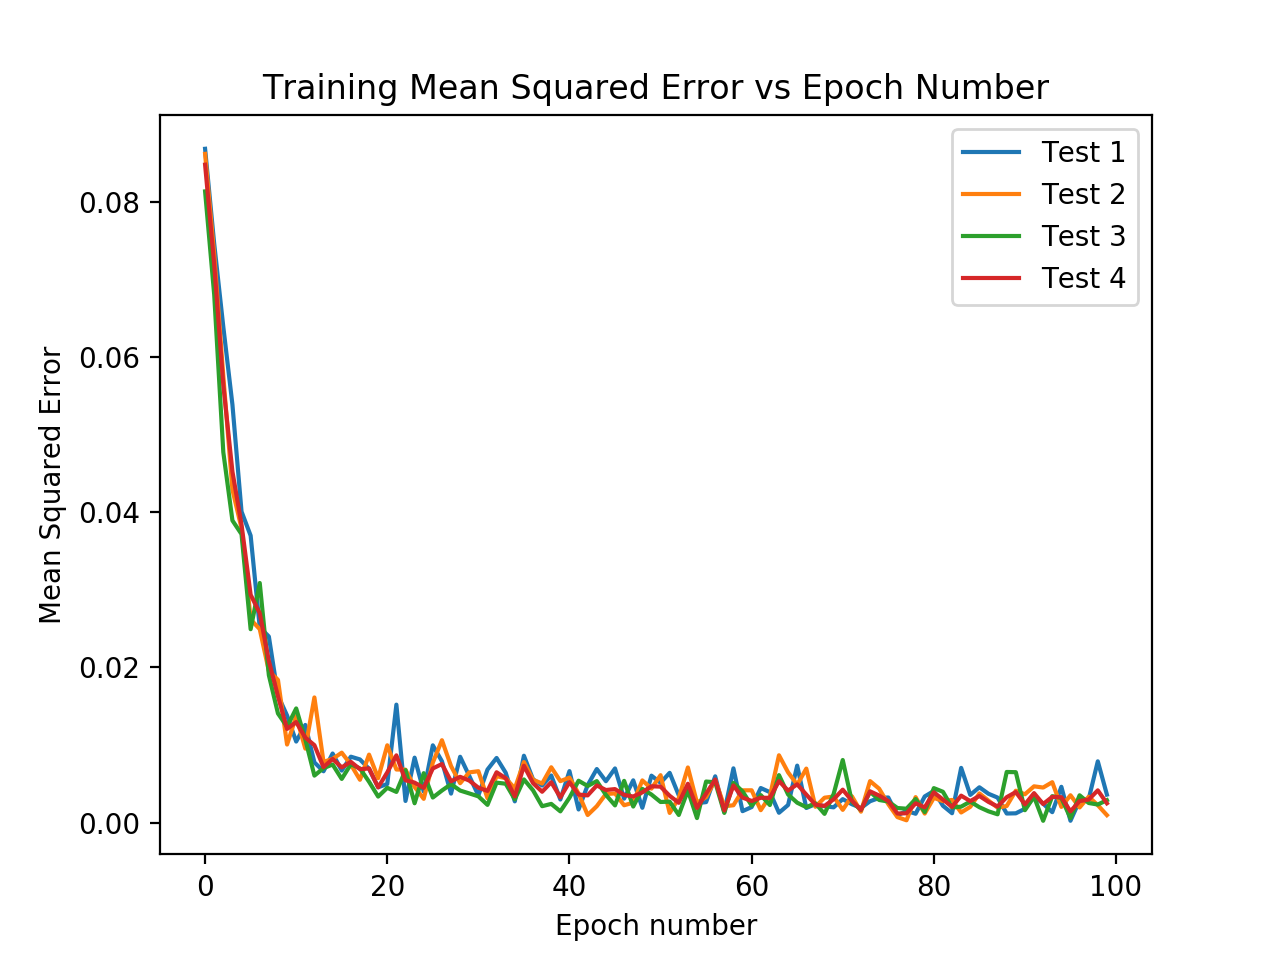
\includegraphics[scale=0.7]{mnist.png}
\caption{Overall trend of the training error rate with increasing epochs.}\label{fig:mnist}
\end{figure}
Figure \ref{fig:mnist} shows the model converges quickly to a low mean squared error rate. Around 20 epochs are required for the changes in further training to be negligible in improving the performance of the model.
\section{Android application}
% Add intro sentence to say why measuring, eg for users battery performance, usability. 
The memory and CPU utilization from the Android Application was retrieved from the Android profiler. The Android profiler is a tool to provide real time data of the applications performance~\cite{profiler}. We get the usage statistics from the different stages of the classification pipeline, from the construction of the edge lists from the location data, the feature extraction from the edge list and then the classification of feature vector constructed. Battery consumption is not an issue since the inference only needs to occur once a week and only executes for around 15 seconds. Also, the device can be plugged in whilst the inference takes place as it can be made anywhere. 
\subsection{Result}
Here I show the screen shots of the Android application to infer the users' occupation class.
\begin{figure}[H]
\centering
\graphicspath{{images/}}
\includegraphics[width=.32\textwidth]{app.jpg}\hfill
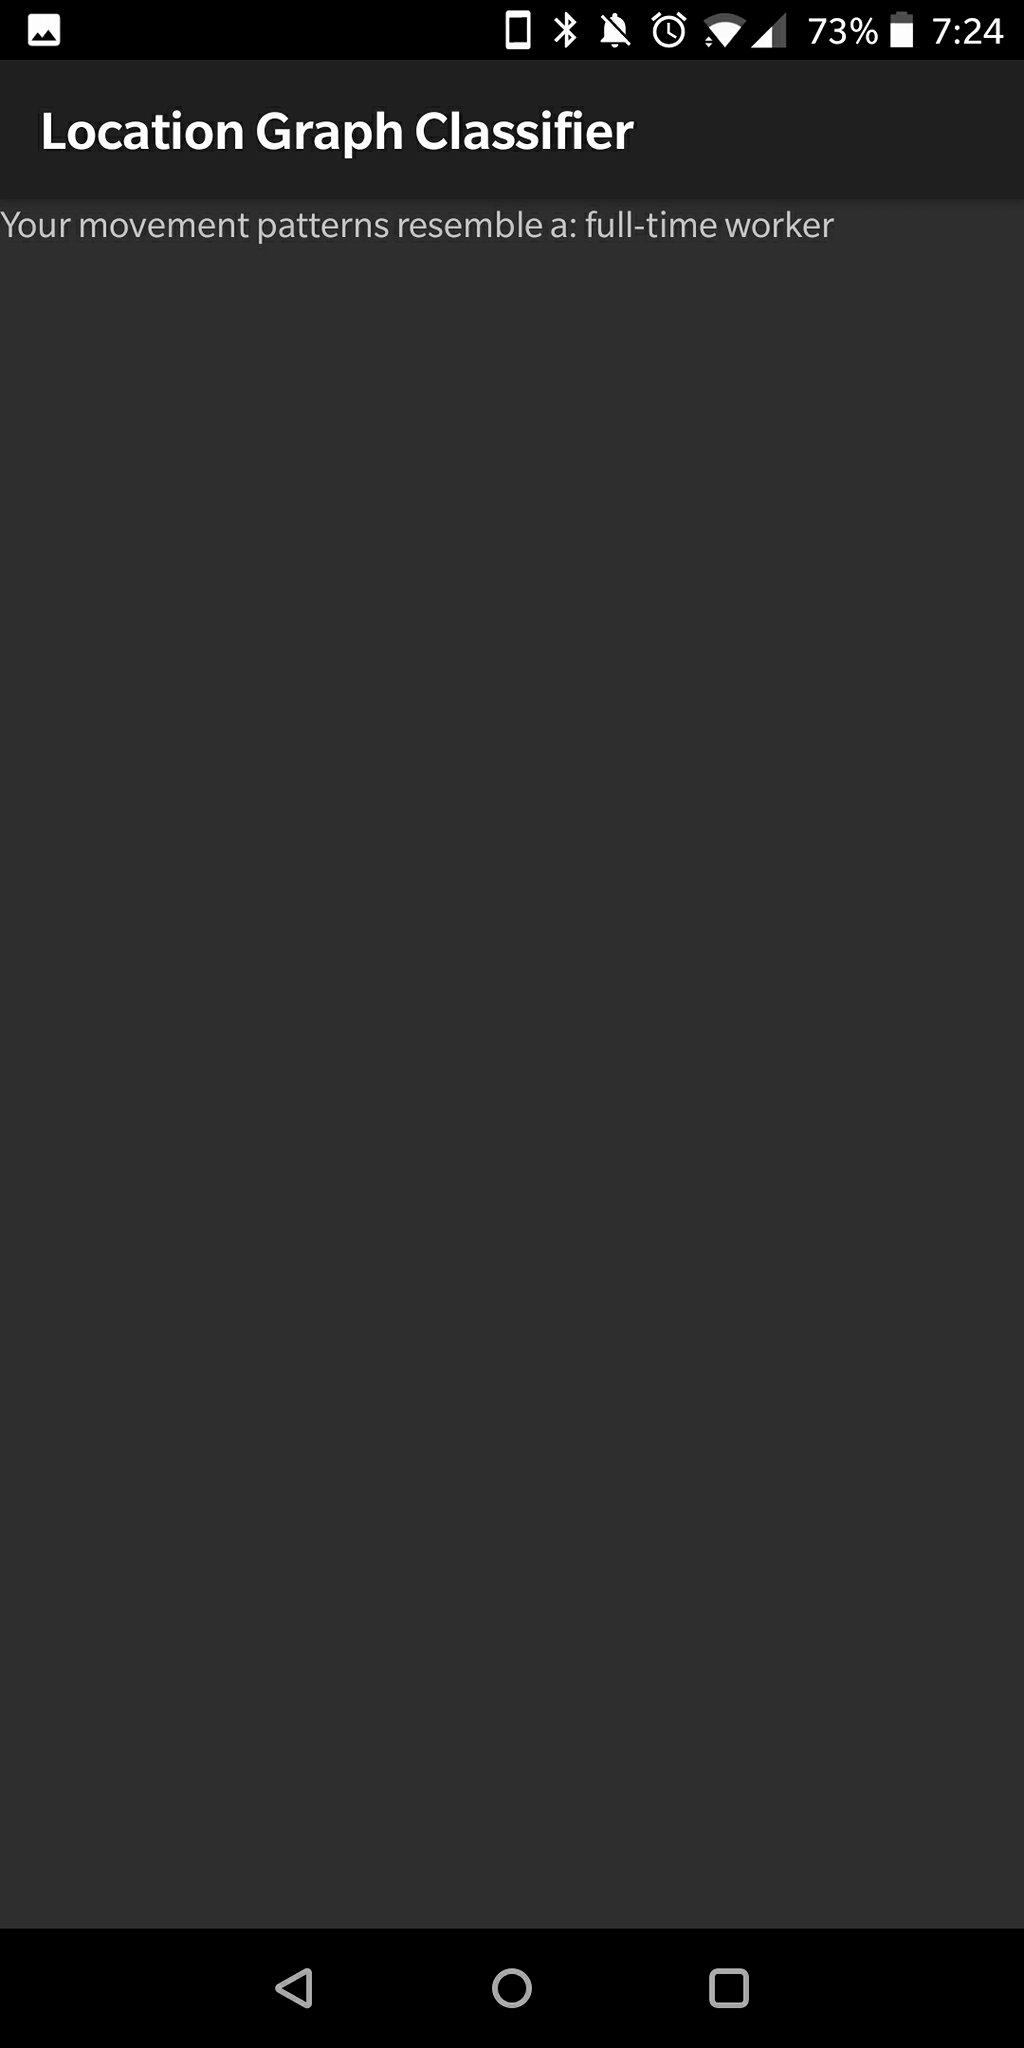
\includegraphics[width=.32\textwidth]{screenshot.jpg}\hfill
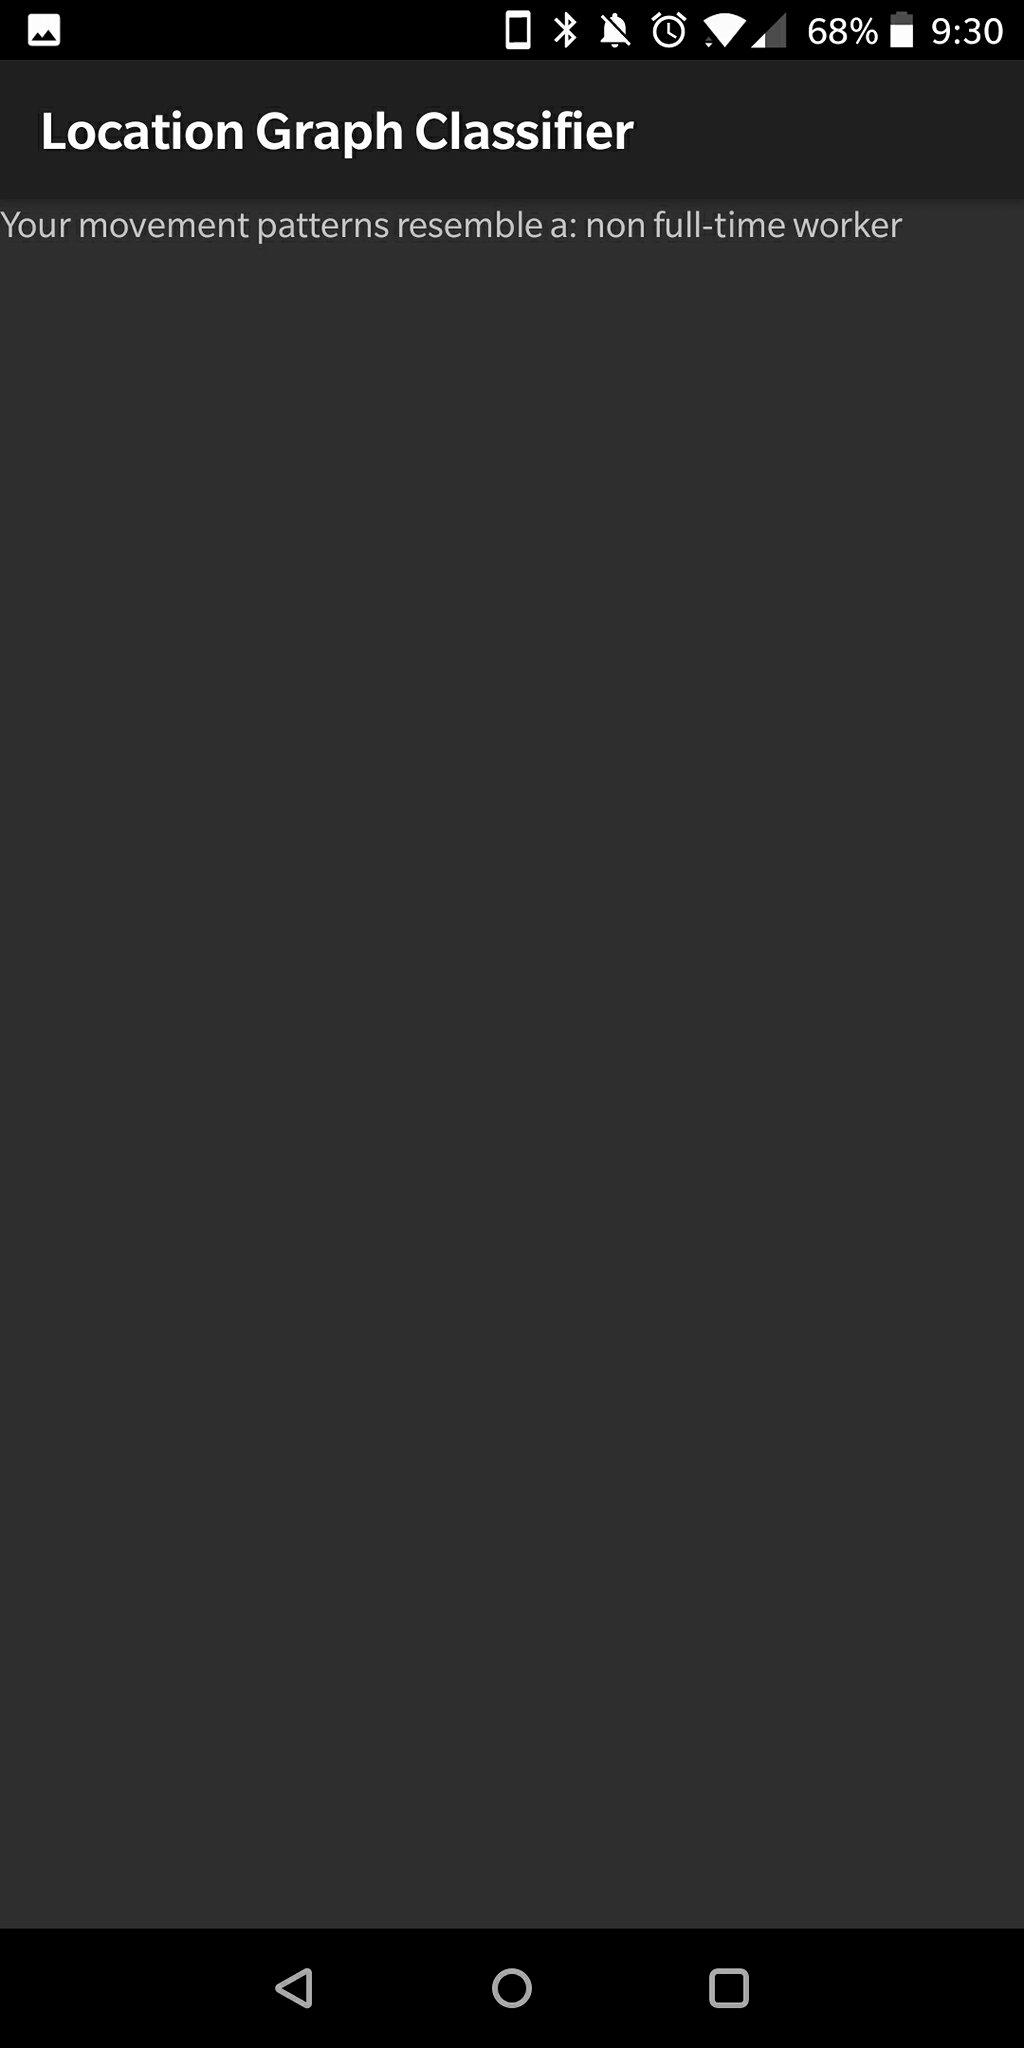
\includegraphics[width=.32\textwidth]{screenshot2.jpg}
\caption{Screenshots of the application start screen and the two types of inferences possible.}
\label{fig:screenshots}
\end{figure}
\subsection{CPU Utilisation}
\graphicspath{{images/}}
\begin{figure}[H]
\centering
\includegraphics[scale=0.6]{time2.png}
\caption{CPU utilisation graph showing the different stages of the application.}\label{fig:cpu}
\end{figure}
The inference takes around 15 seconds to complete for all the stages from building the graph to inference. It is not possible to generate the graph consistently throughout the week since some locations will be discarded from the final graph later on if not visited enough. Also the application is limited to 20\% of the CPU and so is not exceeding its share of the processing power and is not detrimental to the performance of the phone whilst using the application. The first small spike (1) is the opening of the application followed by three stages of the inference: building the graph edge list (2), edge feature extraction (3) then inference (4) as seen by the three different blocks in the am.cl.loclogger thread
\subsection{Memory Utilisation}
\graphicspath{{images/}}
\begin{figure}[H]
\centering
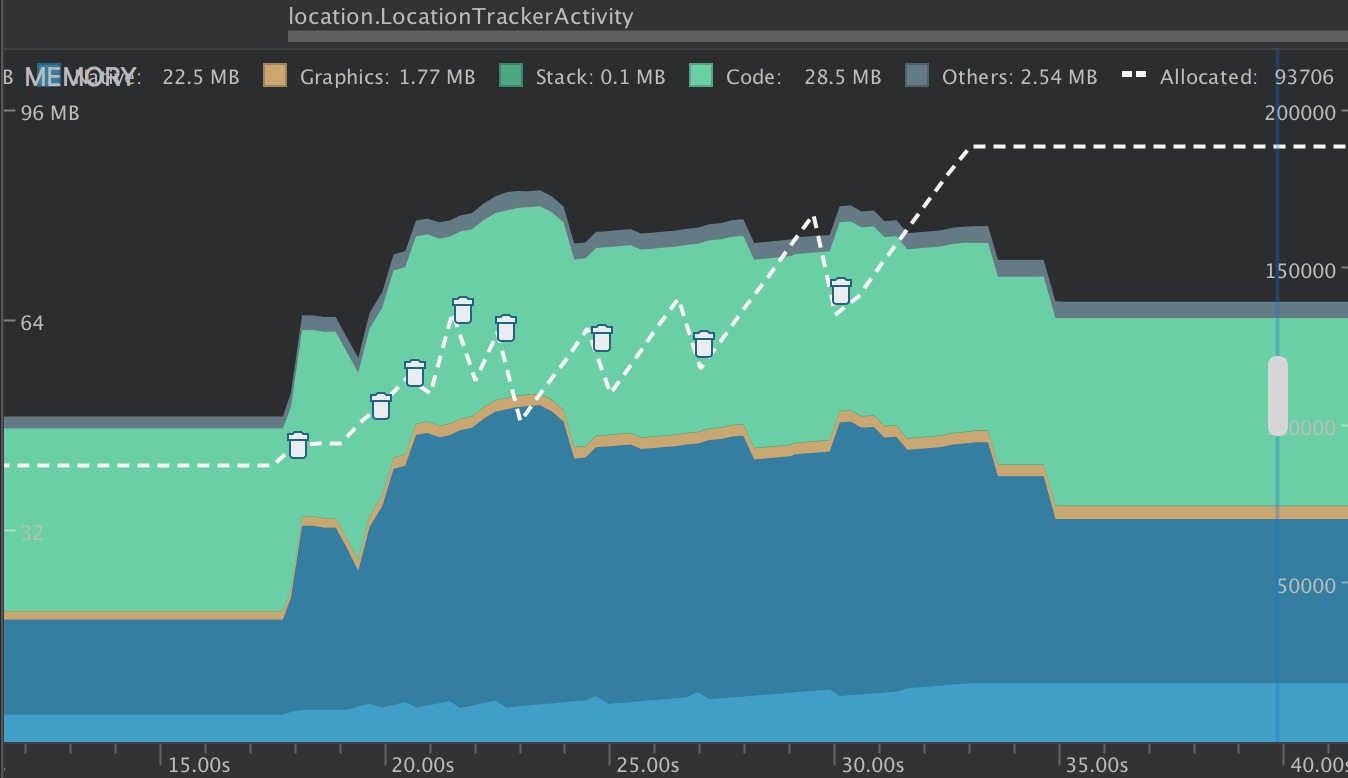
\includegraphics[scale=0.7]{memory.png}
\caption{A graph of the memory consumption of application opening and inference tasks.}\label{fig:memory}
\end{figure}
Figure 4.5 shows that the memory usage is less than 96MB. Given that most recent Android phones have at least 1GB of RAM the application should work on a whole range of phones. There is a large amount of garbage collection that can be seen after the graph edge list has been used, after creating the edge features and after the creating the WEKA feature vector. The de-serialisation of the random forest model then uses up a large amount of memory.
\chapter{Conclusion}
The project was a success, I designed, built and evaluated mobility graphs, several supervised machine learning algorithms and an Android application to meet the success criterias and additional extensions set out earlier. 
\section{Results}
The project success criterias were successfully achieved and surpassed by implementing additional extensions, such as the Neural Network implementation.
% The results obtained highlight that the use of machine learning models to study mobility graphs could be more successful. 
The use of feature extraction on synthetic graph data to make predictions based on the graph edge lists was evaluated to be significant. This indicates that it is possible to classify statistically independent graphs, although the graphs from the spatio-temporal datasets were not of the highest quality, to allow for a high separation accuracy. 
The project provides a novel framework for on-device machine learning based on mobility graphs constructed. This can be extended by simply replacing the classifier to infer other labels to solve different problems. As phones become more powerful and employ dedicated chips for AI tasks we will need new types of application frameworks to exploit mobile sensor data to solve a new class of problems and this project successfully demonstrates the potential of on-device mobility-graphs classification.
\section{Lessons Learned}
This project has given me the opportunity to get familiar with the theoretical and practical sides of machine learning with the exploration and evaluation of different classifiers applied to a unique, unfamiliar type of data in graphs.
An important lesson I will take away from is to look for ways of shortening the time between training and evaluating the models, since training with incorrect parameters or quality of data could be spotted and improved earlier.
Using the iterative development model for this process proved to be crucial. If I were to do the project again, I would have allowed for even more time to try out different techniques to improve quality of the data and the models. This is particularly important for machine-learning projects, where there usually is not a pre-defined sequence of steps.
\section{Further Work}
% There was a large variance between different tests of the algorithms and so the general trends in the model's behaviour could not be easily reasoned about. 
Further work would go towards improving the quality of the data to make improvements to the accuracies of the models. These improvements could come from adding more information to the mobility graphs since a lot of data is removed in the clustering stage; the time information and rare visits are ignored when the locations are clustered.
I would also carry out the other extension specified of creating a distributed machine-learning \cite{distributedml} platform, itself a large undertaking. Finally, more interesting datasets could be applied to the existing algorithms and application easily to infer more interesting classes, such as early Alzheimer's detection. 
\addcontentsline{toc}{chapter}{Bibliography}
\bibliographystyle{abbrv}
% \bibliography{thesis}
\begin{thebibliography}{99}
\bibitem{androido} Android local machine learning applications. 24/4/2018.
https://android-developers.googleblog.com/2017/05/whats-new-in-android-o-developer.html
\bibitem{well-being} S. Servia,  K. Rachuri, C. Mascolo, P. Rentfrow, N. Lathia, G. Sandstrom. Mobile Sensing at the Service of Mental Well-being: a Large-scale Longitudinal Study. SIGCHI conference, 2017.
\bibitem{CNN1} Defferrard, M., Bresson, X.,\& Vandergheynst, P. (2016). Convolutional neural networks on graphs with fast localized spectral filtering. In Advances in Neural Information Processing Systems (pp. 3844-3852).
\bibitem{apple} Smart watch heart disease predictions.  24/4/2018. https://www.apple.com/newsroom/2017/11/apple-heart-study-launches-to-identify-irregular-heart-rhythms/
\bibitem{approximator} Cybenko, G.V.
Approximation by Superpositions of a Sigmoidal function. In van Schuppen, Jan H. Mathematics of Control, Signals, and Systems. Springer International. pp. 303–314. 2006
\bibitem{dataset} Kiukkonen, N., Blom, J., Dousse, O., Gatica-Perez, D., \& Laurila, J. (2010). Towards rich mobile phone datasets: Lausanne data collection campaign. Proc. ICPS, Berlin.
\bibitem{emotion} Rachuri, K., Musolesi, M., Mascolo, C., Rentfrow, P., Longworth, C., Aucinas, A. (2010).
EmotionSense: A Mobile Phones based Adaptive Platform
for Experimental Social Psychology Research.
In Proceedings of the 12th ACM International Conference on Ubiquitous Computing (Ubicomp 2010). Copenhagen, Denmark.
\bibitem{erdos} Erdős, P.; Rényi, A. (1959). "On Random Graphs. I". Publicationes Mathematicae.
\bibitem{cnn} CNN image Source. 24/4/2018. http://adventuresinmachinelearning.com/convolutional-neural-networks-tutorial-tensorflow/
\bibitem{tensorflow}
Abadi, M., Agarwal, A., Barham, P., Brevdo, E., Chen, Z., Citro, C., Corrado, G.S., Davis, A., Dean, J., Devin, M., \& Ghemawat, S. (2016). Tensorflow: Large-scale machine learning on heterogeneous distributed systems. arXiv preprint arXiv:1603.04467.
\bibitem{scikitlearn} Lars Buitinck, Gilles Louppe, Mathieu Blondel, Fabian Pedregosa, Andreas Mueller, Olivier Grisel, Vlad Niculae, Peter Prettenhofer, Alexandre Gramfort, Jaques Grobler, Robert Layton, Jake Vanderplas, Arnaud Joly, Brian Holt, Gaël Varoquaux. API design for machine learning software: experiences from the scikit-learn project. arXiv:1309.0238.
\bibitem{MNIST} MNIST dataset repositor. 24/4/2018. http://yann.lecun.com/exdb/mnist/
\bibitem{nestedcrossvalidation}Cawley, G.C.; Talbot, N.L.C. On over-fitting in model selection and subsequent selection bias in performance evaluation. J. Mach. Learn. Res 2010,11, 2079-2107.
\bibitem{featureselection2}
Bermingham, Mairead L.; Pong-Wong, Ricardo; Spiliopoulou, Athina; Hayward, Caroline; Rudan, Igor; Campbell, Harry; Wright, Alan F.; Wilson, James F.; Agakov, Felix; Navarro, Pau; Haley, Chris S. (2015). "Application of high-dimensional feature selection: evaluation for genomic prediction in man". Sci. Rep. 5.
\bibitem{variance}
Variance threshold feature selection method. 24/4/2018. scikit-learn.org/stable/modules/generated/sklearn.feature\_selection.VarianceThreshold.html
\bibitem{featurescaling}S. Aksoy and R. Haralick, "Feature normalization and likelihood-based similarity measures for image retrieval," Pattern Recognition. Lett., Special Issue on Image and Video Retrieval, 2000.
\bibitem{adam} Diederik P. Kingma, Jimmy Ba. Adam: A Method for Stochastic Optimization. Dec 2014 . arXiv:1412.6980 
\bibitem{dropout} Nitish Srivastava, Geoffrey E Hinton, Alex Krizhevsky, Ilya Sutskever, and Ruslan Salakhutdinov. Dropout: a simple way to prevent neural networks from overfitting. Journal of Machine Learning Research. arXiv:1207.0580. 2014.
\bibitem{NetworkX} Aric A. Hagberg, Daniel A. Schult and Pieter J. Swart, “Exploring network structure, dynamics, and function using NetworkX”, in Proceedings of the 7th Python in Science Conference (SciPy2008), Gäel Varoquaux, Travis Vaught, and Jarrod Millman (Eds), (Pasadena, CA USA), pp. 11–15, Aug 2008
\bibitem{hyperparameter}
Claesen, Marc; Bart De Moor (2015). "Hyperparameter Search in Machine Learning". arXiv:1502.02127.
\bibitem{profiler} Android Profiler. 24/4/2018. developer.android.com/studio/profile/android-profiler.html 
\bibitem{graph2vec} 
Annamalai Narayanan, Mahinthan Chandramohan, Rajasekar Venkatesan, Lihui Chen, Yang Liu, Shantanu Jaiswal (Jul 2017).
graph2vec: Learning Distributed Representations of Graphs. arXiv:1707.05005
\bibitem{distributedml} 
Shokri, R., \& Shmatikov, V. (2015, October). Privacy-preserving deep learning. In Proceedings of the 22nd ACM SIGSAC conference on computer and communications security (pp. 1310-1321). ACM.
\end{thebibliography}
% \appendix
% \printthesisindex
\begin{appendices}
\chapter{Project Proposal}
\begin{center}
\Large
Computer Science Tripos -- Part II -- Project Proposal\\[4mm]
\LARGE
Comparing Machine Learning Techniques for Mobility Graph Classification\\[4mm]
\large
Miteyan Patel, Robinson College\\
Originator: Dr Sandra Servia\\
20th October 2017
\end{center}
\vspace{5mm}
\textbf{Project Supervisor:} Dr Sandra Servia\\
\textbf{Director of Studies:} Prof Alan Mycroft\\
\textbf{Project Overseers:} Dr Ian Wassell \& Dr Rafal Mantiuk
% Main document
\section*{Introduction}
The pervasiveness of smartphones has generated large amounts of data, whose analysis can disclose valuable information regarding users' behaviour. At the same time, recent advances in machine learning, especially on generalising the use of Convolutional Neural Networks (CNN) on graphs, have allowed extending the use of deep learning beyond the NLP and image recognition domains. In this project, we will explore the performance of different machine learning techniques to the task of inferring demographics (age, gender, job type) of the individuals from a graph representation of their mobile GPS location data. The best performing model will be trained on the server and ported to a mobile phone application which collects location data, builds mobility graphs from it and uses the model and graphs to infer the demographics of the user locally on their device. 

The main motivation of the project is to select a machine learning model and provide a mobile framework for classifying users according to their mobility patterns, whilst keeping their location data on their devices in order to prevent privacy leaks. A similar approach has applicability to identifying stages of Alzheimer's Disease given a suitable data set, since it has been observed that getting lost and misremembering the location of places are symptoms that typify the onset of the disease, therefore their mobility graphs are likely to differ from the neurotypical which could be used for early diagnoses of the disease before symptoms such as dementia and irreversible brain damage occur.

Two main issues need to be addressed to build such a system for this project. First, the selection of a supervised classifier to infer the user's demographic label. Recent advances in Machine Learning have generalised CNNs from regular grid-like data such as images and speech to irregular data like graphs as inputs \cite{CNN1,CNN2,CNN3}. For this project, we will explore the use of graph CNNs to infer individuals' demographic label from graph representations of their mobile GPS location data collected with their mobile devices. We will study how graph CNNs compares to traditional supervised learning approaches, from Logistic Regression to Support Vector Machines, based on feature extraction of the graphs. We will evaluate the performance by comparing the memory required, the speed of training and making predictions with the models, and accuracy of the different approaches after optimising each. For the input data into the models, we will create graphs with nodes for locations and edges as transitions between locations in the period of observation.

Second, we need to provide a privacy-aware solution that guarantees the confidentiality of the individual’s sensitive location data and prevent privacy leaks by inferring the label locally on the mobile device. To do so, we will build and train the model on a server by using the dataset. This model will be then ported to a mobile phone application that collects the location data, builds the graph and infers the demographic label locally. We will also evaluate the performance of the model on the mobile application regarding its time to build location graphs and infer the users class, as well as the battery consumption.
\section*{Starting point}
I have previous knowledge about machine learning through the \textbf{Artificial Intelligence} course and reading in my spare time, although for a deeper understanding of the machine learning algorithms and knowledge about making optimizations for increasing the performance of the algorithms I aim to use the Machine Learning by Stanford online course\cite{MLcourse}. There is also a \textbf{Machine Learning and Bayesian Inference} course in Lent. Although I intend to complete most of the work concerning these algorithms before the start of the course and learn about other additional algorithms from other sources. I have previous knowledge of Python, TensorFlow, Scikit-learn \cite{tensorflow,scikitlearn} through small projects and reading, although I aim to improve these skills through the online resources such as the Deep Learning courses on Udacity and Coursera\cite{udacity, coursera}. I also intend to read relevant papers, blog posts, videos to further understanding. \textbf{Algorithms}, \textbf{Software Engineering}, \textbf{OOP}, \textbf{Mathematical Methods for Computer Science} are courses that will be useful throughout the project.\\

I will be using the Nokia: The Mobile Data Challenge: Big Data for Mobile Computing Research dataset\cite{dataset} containing location in latitude longitude collected from smartphone GPS sensors in Lausanne, Switzerland, for over a year. It contains demographic labels such as gender, age group, marital status, job type, and number of people in the household for some users.\\

I will be investigating the potential of a recent paper: Convolutional Neural Networks on Graphs with Fast Localized Spectral Filtering \cite{CNN1}. It contains an implementation which I will be modifying for use on the mobility graphs constructed because it would be difficult to implement a better version from scratch and therefore will give me better results, whilst allowing me more time to try out other possible traditional algorithms and determine if we need the advanced graph CNN algorithm to accurately predict a users class or if we could just use feature extraction and standard supervised classifiers for a similar testing error and compare the trade-offs. The implementation will be used under the MIT license and the paper will be cited\cite{CNN1}. \\

I will use an existing script to extract graphs from raw GPS data from the Nokia dataset to start with. This will allow me to earlier address the main aims of the project, leaving the investigation of how to build better trajectory graphs from GPS traces as a possible extension for this project. There is an application for Android that collects GPS location coordinates that will be greatly extended to build graphs, extract possible features and  infer the users class.\\
\textbf{Libraries}
\begin{itemize}
\item Android SDK: Development environment for Android. I am already familiar with this from previous projects and the group project.
\item TensorFlow \cite{tensorflow}: Open source deep learning library, to assist in the implementation of the algorithms and used in the graph CNN paper. TensorFlow is widely used in industry and research as the CNN paper uses TensorFlow \cite{CNN1} so my understanding of TensorFlow is paramount to understand and modification of the open source implementation, it also allows a model to be ported to Android. 
\item Scikit-learn \cite{scikitlearn}: Another machine learning library. Will allow experimenting with more algorithms and are optimized for faster training and would work better than an implementation from scratch, also contains API for porting to Android. This will help meet my success criterias earlier and possibly allow the extensions to be implemented.\end{itemize}
\section*{Resources required}
The project will be carried out on my personal laptop, a mid 2014 MacBook Pro running macOS Sierra. However, the computation will be done in the server \textit{pizza.cl.cam.ac.uk} that I will be given access to for the use of the restricted dataset\cite{dataset}. I also have my own Android Nexus 5X smart phone which I can use to test and build the application. If it breaks I will get a new Android phone.\\
The dataset is available only for use on this server, I have permission to access the server and dataset from my supervisor and through the system administrators at the Computer Lab. The University has an agreement in place to use the data until December 2018. I have signed a Confidentiality Disclosure Agreement with Idiap Research Institute for the use of the dataset and adhere to the strict rules about the restricted data and its privacy.
I will have get approval for the ethical review of research with human participants for the use of personal information from the dataset and also for potential tests of the application for Android if time permits.

I will use a GitHub repository, with separate branches for the mainline, features and bug fixed for organising the project and to commit code only a few hours after completion to prevent losing more than a few hours of code in case my machine breaks. It also allows the ability to track bugs, control versions, and host the code in a safe, easily accessible place in case my machine breaks. I will also make backups every major update onto several USB sticks.\\\\\\

\section*{Work to be done}

The project breaks down into the following sub-projects:
\begin{enumerate}
\item  Understanding the graph CNN algorithm proposed in \cite{CNN1} and modifying the open source implementation accordingly, as well as the input pipeline to classify the location graphs. These graphs will be previously extracted from the Mobile Challenge Dataset location data \cite{dataset} and divided into training, validation and test set.
\item Identifying relevant features from the mobility graphs that will be used for inputs into the supervised learning algorithms. These will be different measurements of centrality, shortest path, centrality, etc.
\item Implementing  machine learning algorithms in Python using TensorFlow and scikit-learn\cite{tensorflow, scikitlearn}. These will use, as input data, the relevant feature identified in 2. These may include the following but are not limited to and likely to change: Logistic Regression, Support Vector Machines, Naive Bayes classifier, Neural Networks, Decision Trees, Random Forests. 
\item Optimising the different trained models for accuracy, time and space. Identifying the best performing model to be ported to the mobile phone application.
\item Modifying the implementation for use in the Android mobile phone application using the TensorFlow Android API and completing the Android app to construct graphs locally from the location data and use the model to locally infer the label. Evaluate the time it takes for the building of the graph from location data, the time it takes to make the class inference for the user, as well as the battery consumption.

\end{enumerate}
\section*{Success criteria}
 At the end of the project I should have completed the following criteria to allow the project to be considered successful:
\begin{enumerate}
\item Applied, optimized and tested the graph CNN algorithm to the location graphs constructed from raw location data to classify the user into their demographic class\cite{CNN1}.
\item Trained, optimized, and benchmarked the performance of the supervised machine learning algorithms on features extracted from mobility graphs.
\item Evaluated the models quantitatively and chosen the most appropriate of these and pre-train the model and port into the Android application. 
\item Have an Android application which can construct mobility graphs from the users location and infer the demographic class of the user locally using the model.

\end{enumerate}
\section*{Possible extensions}

If I achieve my main result early, I will explore how to construct different types of graphs from the raw location data. The nodes can be represented as either latitude and longitude pair or an area of the coordinates. The edges could include the direction of the user or be undirected. We could also add weights to edges based on popularity of the location, or omit less popular or more popular locations. Other possibility would be to create synthetic data for Alzheimer's patients based on differences in movements between people with memory impairing diseases such as Alzheimer’s disease and the neurotypical, by sensing changes in their tracking graph for early diagnosis.  I might also use the graph2vec \cite{graph2vec} algorithm to convert the graphs created into a vector which can be directly used by the traditional machine learning algorithms, or try other graph CNN algorithms \cite{CNN2,CNN3}, although their open source implementation has not been released yet.\\

Further extensions could include creating a distributed machine learning model\cite{distributedml}, where the model would be trained cooperatively and successive updates of the model would happen locally on the users' devices. This would ensure the confidentiality of the location data since it is not sent to a server, but only the weights of the trained model are disclosed. However, this would involve many changes and extensions to the existing system and therefore it may be more appropriate as future work after the dissertation time frame.\\

\section*{Timetable}
\begin{itemize}
\item \textbf{Michaelmas weeks 0-2 | October 6th - 20th}\\
- Refine the project idea and write project proposal drafts.\\
- Make changes to draft and project based on feedback.\\
\textbf{Milestones:} Have a finished Project Proposal submitted by October 20th.
\item \textbf{Michaelmas weeks 2-4 | October 21st - November 3rd}\\
- Background reading on TensorFlow, Scikit-learn, supervised machine learning techniques, Naive Bayes classifier, SVM, Neural Networks, Decision Trees, graph feature extractions, graph CNN algorithms\\
- Set up GitHub repository, back up storage solutions for the project in case of failures.\\
\textbf{Milestones: }Studied the online courses\cite{MLcourse,udacity,coursera} and background reading needed for the theory and skills to complete the project. 
\item \textbf{Michaelmas weeks 4-6 | November 4th - 17th}\\
- Construct graphs from raw location data.\\
- Split into training and test sets.\\
- Create a dissertation layout LATEX document.\\
- Read the graph CNN paper\cite{CNN1}.\\
\textbf{Milestones: }Have working training, test, validation datasets for the graph CNN algorithm. Understood the graph CNN algorithm.\\


\textbf{Michaelmas weeks 6-8| November 18th - December 1st}\\
- Modify the Graph CNN algorithm for the location graph dataset.\\
\textbf{Milestones:} Started working on training model for the graph CNN.
\item \textbf{Christmas vacation weeks 0-2 | December 2nd - 15th}\\
- Continue work on the graph CNN and train, optimize, benchmark, evaluate.\\
- Extract Features from graphs for traditional supervised learning tasks and make test, train, validation dataset.\\
- Start writing up the Introduction chapter.\\
\textbf{Milestones: }Finished and have a working trained model for the graph CNN and so have met the first success criteria. Have working training, test, validation datasets to allow development of machine learning algorithms.
\item \textbf{Christmas vacation weeks 2-4 | December 16th - 29th}\\
- Implement, train, optimise, test Naive Bayes, Logistic Regression and Neural Network classifiers.\\
- Start writing Preparation chapter.\\
\textbf{Milestones: }Have working Naive Bayes, Logistic Regression and Neural Network models with metrics for training data to allow for evaluation later on. Finished writing the introduction chapter draft.
\item \textbf{Christmas vacation weeks 4-6 | December 30th - January 12th}\\
- Implement, train, optimise, test SVM, Decision Tree, Random Forest classifiers, or other through research.\\
\textbf{Milestones: }Have working SVM, Decision Tree, Random Forest  models for training data with metrics to allow for evaluation later on. Finished the preparation chapter.
\item \textbf{Lent weeks 0-2 | January 13th - 26th}\\
- Evaluate and compare all of the machine learning models.\\
- Start creating application for Android to construct graph from location data then infer the class of the user. \\
- Started writing the implementation chapter.\\
 \textbf{Milestones: }Evaluated and chosen the best machine learning model to be exported to the Android application and so have met the second success criteria. Finished the preparation chapter draft.
\item \textbf{Lent weeks 2-4 | January 27th - February 9th}\\
- Start, complete and send the progress report by February 2nd and be ready for the overseers presentation. \\
- Make and practice the overseers presentation.\\
- Train and export machine learning model to application to make predictions locally.\\
\textbf{Milestones:} Sent the progress report and have practiced the presentation to overseers. Exported the best model to Android, using TensorFlow Android API or scikit-learn open source API \cite{tensorflow,skitlearnandroid}, to port pre-trained model and met the third success criteria.
\item \textbf{Lent weeks 4-6 | February 10th - February 23rd}\\
- Complete, test and debug the application for Android.\\
- Start writing the evaluation chapter.\\
\textbf{Milestones: }Tested the application to make predictions the application for Android and met the last success criteria. Finished writing the implementation chapter. \\
\item \textbf{Lent weeks 6-8| February 24th - March 9th}\\
- Finish up any existing implementation work and extensions.\\
- Start writing conclusion.\\
\textbf{Milestones:} Finished up any implementation and extension work for the dissertation.  Finished evaluation chapter.
\item \textbf{Easter vacation weeks 0-2 | March 10th - 23rd}\\
- Buffer slot for delays, testing and work due and potentially for implementing extensions if time permits.\\
- Finish dissertation draft and send to my supervisor and DoS for initial feedback.\\
\textbf{Milestones: } In case of delays not planned for encountered during the project. Submitted a dissertation draft for initial review.
\item \textbf{Easter vacation weeks 2-4 | March 24th - April 6th}\\
- Make changes for the dissertation from comments.\\
\textbf{Milestones:} Updated dissertation based on comments from DoS and supervisor.
\item \textbf{Easter vacation weeks 4-6 | April 7th - 20th}\\
-  Buffer slot in case of delays.\\
- Finish writing dissertation.\\
\textbf{Milestones: }Finished dissertation and ready for hand-in.
\item \textbf{Easter term weeks 0-2 | April 21st - May 4th}\\
- Buffer slot in case of delays.\\
- Submit dissertation.\\
\textbf{Milestones: }Handed in the dissertation by May 4th for the deadline on May 18th.
\end{itemize}
\begin{thebibliography}{9}
\bibitem{CNN1} Defferrard, M., Bresson, X.,\& Vandergheynst, P. (2016). Convolutional neural networks on graphs with fast localized spectral filtering. In Advances in Neural Information Processing Systems (pp. 3844-3852).
\bibitem{CNN2} Niepert, M., Ahmed, M.,
\& Kutzkov, K. (2016, June). Learning convolutional neural networks for graphs. In International Conference on Machine Learning (pp. 2014-2023).
\bibitem{CNN3} Levie, R., Monti, F., Bresson, X., \& Bronstein, M. M. (2017). CayleyNets: Graph Convolutional Neural Networks with Complex Rational Spectral Filters. arXiv preprint arXiv:1705.07664.
\bibitem{MLcourse} Stanford University: Machine Learning course \\\texttt{https://www.coursera.org/learn/machine-learning}
\bibitem{udacity} Deep Learning Python TensorFlow course 
\\\texttt{https://www.udacity.com/course/deep-learning--ud730}
\bibitem{coursera} Deep Learning Python sklearn course 
\\\texttt{https://www.coursera.org/learn/neural-networks-deep-learning/}
\bibitem{dataset} Kiukkonen, N., Blom, J., Dousse, O., Gatica-Perez, D., \& Laurila, J. (2010). Towards rich mobile phone datasets: Lausanne data collection campaign. Proc. ICPS, Berlin.
\bibitem{tensorflow}
Abadi, M., Agarwal, A., Barham, P., Brevdo, E., Chen, Z., Citro, C., Corrado, G.S., Davis, A., Dean, J., Devin, M., \& Ghemawat, S. (2016). Tensorflow: Large-scale machine learning on heterogeneous distributed systems. arXiv preprint arXiv:1603.04467.
\bibitem{scikitlearn} Lars Buitinck, Gilles Louppe, Mathieu Blondel, Fabian Pedregosa, Andreas Mueller, Olivier Grisel, Vlad Niculae, Peter Prettenhofer, Alexandre Gramfort, Jaques Grobler, Robert Layton, Jake Vanderplas, Arnaud Joly, Brian Holt, Gaël Varoquaux. API design for machine learning software: experiences from the scikit-learn project. arXiv:1309.0238.
\bibitem{skitlearnandroid} Scikit-learn porter for Java \\
\\\texttt{https://github.com/nok/sklearn-porter}
\bibitem{graph2vec} 
Annamalai Narayanan, Mahinthan Chandramohan, Rajasekar Venkatesan, Lihui Chen, Yang Liu, Shantanu Jaiswal (Jul 2017).
graph2vec: Learning Distributed Representations of Graphs. arXiv:1707.05005
\bibitem{distributedml} 
Shokri, R., \& Shmatikov, V. (2015, October). Privacy-preserving deep learning. In Proceedings of the 22nd ACM SIGSAC conference on computer and communications security (pp. 1310-1321). ACM.
% \\\texttt{http://cs.brown.edu/~agg/EDBS.pdf}
\end{thebibliography}
\end{appendices}
\end{document}